\section{A taxonomy of robot-evaluation benchmarks}
\label{sec:taxonomy}

Figure~\ref{fig:taxonomy_main} organises 86 representative benchmarks under a single root and four
evaluation lanes. The lanes are ordered by how close their scoring sits to executed behaviour: from
closed-loop policy suites (Section~\ref{sec:taxonomy} \S3.1) and embodied-agent benchmarks (\S3.2),
through open-loop world-model evaluation (\S3.3), to the prediction-to-action bridges (\S3.4) that
alone turn prediction into action. Within each lane, benchmarks are grouped by the capability they
stress. Table~\ref{tab:compare_main} gives a detailed comparison of a representative subset on
year, venue, evaluation mode, and contrast, and Table~\ref{tab:matrix} places one exemplar per lane
against a common set of capability dimensions; neither lane's exemplar builds the VLA-versus-world-model
contrast that Section~\ref{sec:gap} isolates.

% HERO taxonomy -- AUTO-GENERATED by no_upload/gen_taxonomy_p3.py; do not hand-edit.
\begin{figure*}[p]
\centering
\resizebox{!}{0.9\textheight}{%
\begin{forest}
  for tree={align=center},
  where level=0{font=\Large, text width=10.5em}{},
  where level=1{font=\large, text width=13em}{},
  where level=2{font=\normalsize, text width=12.5em}{},
  where level=3{font=\footnotesize, text width=33em, align=left}{},
[\textbf{Robot-evaluation}\\\textbf{benchmarks for}\\\textbf{predictive}\\\textbf{embodied AI}, fill=tx-root, text width=10.5em
  [\textbf{\S3.1 Policy suites}, fill=cat-vla
    [\textbf{\S3.1.1 Manipulation}, fill=cat-vla
      [{\textbf{ARNOLD}: language-grounded continuous-state 3D manipulation~\citep{arnold}\\\textbf{BiGym}: mobile bimanual manipulation~\citep{bigym}\\\textbf{FMB}: real-world functional multi-step assembly manipulat\ldots~\citep{fmb}\\\textbf{Franka Kitchen}: multi-task kitchen manipulation~\citep{frankakitchen}\\\textbf{FurnitureBench}: real-world furniture assembly~\citep{furniturebench}\\\textbf{GRUtopia}: city-scale embodied navigation and manipulation~\citep{grutopia}\\\textbf{ManiSkill2}: generalizable skills~\citep{maniskill2}\\\textbf{PerAct}: language-conditioned 6-DoF single-arm manipulation~\citep{peract}}, fill=leaf-vla]
    ]
    [\textbf{\S3.1.2 Generalization}, fill=cat-vla
      [{\textbf{GemBench}: generalization levels~\citep{gembench}\\\textbf{LIBERO}: short-horizon + transfer~\citep{libero}\\\textbf{RoboArena}: real-world generalization~\citep{roboarena}\\\textbf{SIMPLER / SimplerEnv}: generalization (real vs sim)~\citep{simpler}\\\textbf{THE COLOSSEUM}: generalization / robustness~\citep{thecolosseum}\\\textbf{VIMA-Bench}: multimodal-prompt generalization~\citep{vimabench}}, fill=leaf-vla]
    ]
    [\textbf{\S3.1.3 Other}, fill=cat-vla
      [{\textbf{CortexBench}: pretrained visual representations for embodied cont\ldots~\citep{cortexbench}\\\textbf{GenManip}: LLM-scene tasks~\citep{genmanip}\\\textbf{HandoverSim}: human-to-robot object handover~\citep{handoversim}\\\textbf{Meta-World}: multi-task / meta-RL~\citep{metaworld}\\\textbf{RoboHive}: unified robot-learning environments~\citep{robohive}}, fill=leaf-vla]
    ]
    [\textbf{\S3.1.4 Dexterous}, fill=cat-vla
      [{\textbf{Bi-DexHands}: bimanual dexterous manipulation~\citep{bidexhands}\\\textbf{DexArt}: dexterous articulated-object manipulation~\citep{dexart}\\\textbf{UniDexGrasp}: universal dexterous grasping~\citep{unidexgrasp}\\\textbf{DeformableGym}: 3D deformable-object grasping}, fill=leaf-vla]
    ]
  ]
  [\textbf{\S3.2 Embodied agents}, fill=cat-code
    [\textbf{\S3.2.1 Long-horizon}, fill=cat-code
      [{\textbf{Alexa Arena}: task-planning~\citep{alexaarena}\\\textbf{ALFRED}: long-horizon, partial-obs~\citep{alfred}\\\textbf{BEHAVIOR-1K}: long-horizon household~\citep{behavior1k}\\\textbf{CoELA (C-WAH/TDW-MAT)}: long-horizon~\citep{coela}\\\textbf{DialFRED}: task-planning~\citep{dialfred}\\\textbf{EgoPlan-Bench}: task-planning~\citep{egoplanbench}\\\textbf{EmbodiedBench}: long-horizon~\citep{embodiedbench}}, fill=leaf-code]
    ]
    [\textbf{\S3.2.2 Social \& multi-agent}, fill=cat-code
      [{\textbf{CrowdNav}: social~\citep{crowdnav}\\\textbf{Habitat 3.0}: social / multi-agent~\citep{habitat30}\\\textbf{HuNavSim}: social~\citep{hunavsim}\\\textbf{JRDB}: social~\citep{jrdb}\\\textbf{JRDB-Act}: social~\citep{jrdbact}\\\textbf{Melting Pot}: social~\citep{meltingpot}\\\textbf{Overcooked-AI}: social~\citep{overcookedai}}, fill=leaf-code]
    ]
    [\textbf{\S3.2.3 Navigation}, fill=cat-code
      [{\textbf{Gibson Env}: navigation~\citep{gibsonenv}\\\textbf{GOAT-Bench}: multi-modal lifelong navigation~\citep{goatbench}\\\textbf{Habitat}: navigation~\citep{habitat}\\\textbf{Habitat 2.0}: rearrangement~\citep{habitat20}\\\textbf{HM3D}: navigation~\citep{hm3d}\\\textbf{iGibson}: interactive navigation~\citep{igibson}\\\textbf{Matterport3D}: navigation~\citep{matterport3d}}, fill=leaf-code]
    ]
    [\textbf{\S3.2.4 Autonomous driving}, fill=cat-code
      [{\textbf{Bench2Drive}: driving~\citep{bench2drive}\\\textbf{CARLA}: driving~\citep{carla}\\\textbf{DriveArena}: driving~\citep{drivearena}\\\textbf{MetaDrive}: driving~\citep{metadrive}\\\textbf{NAVSIM}: driving~\citep{navsim}\\\textbf{nuScenes}: driving~\citep{nuscenes}\\\textbf{Waymax}: driving~\citep{waymax}}, fill=leaf-code]
    ]
    [\textbf{\S3.2.5 Counterfactual}, fill=cat-code
      [{\textbf{ACRE}: counterfactual~\citep{acre}\\\textbf{CausalCity}: counterfactual~\citep{causalcity}\\\textbf{CausalVQA}: counterfactual~\citep{causalvqa}\\\textbf{CausalWorld}: counterfactual~\citep{causalworld}\\\textbf{CoPhy}: counterfactual~\citep{cophy}\\\textbf{CRAFT}: counterfactual~\citep{craft}\\\textbf{Filtered-CoPhy}: counterfactual~\citep{filteredcophy}}, fill=leaf-code]
    ]
    [\textbf{\S3.2.6 Locomotion}, fill=cat-code
      [{\textbf{Barkour}: legged locomotion~\citep{barkour}\\\textbf{Brax}: locomotion~\citep{brax}\\\textbf{DERL}: locomotion~\citep{derl}\\\textbf{HumanoidBench}: humanoid locomotion~\citep{humanoidbench}\\\textbf{Isaac Gym}: locomotion~\citep{isaacgym}\\\textbf{Legged Gym}: legged locomotion~\citep{leggedgym}}, fill=leaf-code]
    ]
  ]
  [\textbf{\S3.3 World-model eval}, fill=cat-skill
    [\textbf{\S3.3.1 Generation quality}, fill=cat-skill
      [{\textbf{CATER}: compositional-action temporal reasoning~\citep{cater}\\\textbf{DEVIL}: content-dynamics quality of T2V models~\citep{devil}\\\textbf{EVA-Bench}: embodied video anticipation~\citep{evabench}\\\textbf{EvalCrafter}: generation quality (17-metric suite)~\citep{evalcrafter}\\\textbf{EWMBench}: scene/motion/semantic quality~\citep{ewmbench}\\\textbf{FETV}: fine-grained text-to-video quality~\citep{fetv}\\\textbf{IPV-Bench}: impossible-video generation + understanding~\citep{ipvbench}\\\textbf{StoryBench}: continuous story visualization~\citep{storybench}}, fill=leaf-skill]
    ]
    [\textbf{\S3.3.2 Physical reasoning}, fill=cat-skill
      [{\textbf{ContPhy}: continuum (soft-body/fluid) physical reasoning~\citep{contphy}\\\textbf{GRASP}: grounding + intuitive physics in video MLLMs~\citep{grasp}\\\textbf{IntPhys}: intuitive physics (violation-of-expectation)~\citep{intphys}\\\textbf{IntPhys 2}: intuitive physics in complex scenes~\citep{intphys2}\\\textbf{PHYBench}: physical perception and reasoning~\citep{phybench}\\\textbf{PhyGenBench}: physical-commonsense correctness in video gen~\citep{phygenbench}\\\textbf{PhysBench}: physical-world understanding for VLMs~\citep{physbench}\\\textbf{Physics-IQ}: physical realism~\citep{physicsiq}}, fill=leaf-skill]
    ]
    [\textbf{\S3.3.3 Counterfactual}, fill=cat-skill
      [{\textbf{CLEVRER}: physical/causal video reasoning (counterfactual)~\citep{clevrer}\\\textbf{WorldPrediction}: counterfactual action recognition~\citep{worldprediction}}, fill=leaf-skill]
    ]
    [\textbf{\S3.3.4 Autonomous driving}, fill=cat-skill
      [{\textbf{Vista}: driving world model~\citep{vista}}, fill=leaf-skill]
    ]
  ]
  [\textbf{\S3.4 Bridges}, fill=secE
    [\textbf{\S3.4.1 Other}, fill=secE
      [{\textbf{RoboWM-Bench}: prediction executability~\citep{robowmbench}\\\textbf{World-in-World}: closed-loop task success of WMs~\citep{worldinworld}\\\textbf{WorldArena}: closed-loop WM arena~\citep{worldarena}}, fill=secEl]
    ]
  ]
]
\end{forest}}
\caption{\textbf{A taxonomy of robot-evaluation benchmarks for predictive embodied intelligence} (86 representative benchmarks of the 160 in Table~\ref{tab:landscape}). Each sub-family is one cell listing its benchmarks, each with a short statement of what it measures. Benchmarks are grouped by evaluation lane (\S3.1--\S3.4) and then by the capability they stress. The lanes run from closed-loop task-success suites to the \emph{bridge} frontier (shaded), the only lane that turns prediction into executed action, which is the survey's novelty axis. Full per-benchmark detail: Tables~\ref{tab:compare_main}, \ref{tab:landscape}.}
\Description{A tree diagram organising representative robot-evaluation benchmarks under the root ``robot-evaluation benchmarks for predictive embodied AI'' into four evaluation lanes (policy and manipulation suites; embodied navigation, planning and social; world-model and video-generation evaluation; and prediction-to-action bridges), each split into capability clusters whose cells list benchmarks with what each measures.}
\label{fig:taxonomy_main}
\end{figure*}

% Table -- representative-benchmark comparison, grouped by evaluation lane.
% AUTO-GENERATED by no_upload/gen_compare_main_p3.py; do not hand-edit.
{\footnotesize
\setlength{\tabcolsep}{5pt}
\renewcommand{\arraystretch}{1.15}
\begin{longtable}{@{}p{0.22\textwidth} c l c >{\raggedright\arraybackslash}p{0.30\textwidth} c@{}}
\caption{\textbf{Detailed comparison of a representative 31 of the 160 benchmarks} in the landscape (Table~\ref{tab:landscape}), grouped by evaluation lane. \textbf{Eval}: \dopen\ open-loop prediction/generation quality, \dclosed\ closed-loop task success, \dbridge\ prediction-to-action bridge. \textbf{VLA vs WM}: \yy\ native direct-policy vs world-model contrast, \pp\ partial, \dm\ model-agnostic. Venues are web-verified; ``arXiv'' marks preprint-only works.}\label{tab:compare_main}\\
\toprule
\textbf{Benchmark} & \textbf{Year} & \textbf{Venue} & \textbf{Eval} & \textbf{Capability} & \textbf{VLA vs WM}\\
\midrule
\endfirsthead
\multicolumn{6}{@{}l}{\footnotesize\emph{Table~\ref{tab:compare_main} (continued)}}\\
\toprule
\textbf{Benchmark} & \textbf{Year} & \textbf{Venue} & \textbf{Eval} & \textbf{Capability} & \textbf{VLA vs WM}\\
\midrule
\endhead
\bottomrule
\endlastfoot
\multicolumn{6}{@{}l}{\rule{0pt}{2.6ex}\textbf{\textsf{\S3.1 Policy / manipulation suites}} \hfill \dclosed}\\[1pt]
\textbf{CALVIN}~\cite{calvin} & 2021 & RA-L & \dclosed & long-horizon language & \dm\\
\textbf{LIBERO}~\cite{libero} & 2023 & NeurIPS D\&B & \dclosed & short-horizon + transfer & \dm\\
\textbf{Meta-World}~\cite{metaworld} & 2020 & CoRL & \dclosed & multi-task / meta-RL & \dm\\
\textbf{ManiSkill2}~\cite{maniskill2} & 2023 & ICLR & \dclosed & generalizable skills & \dm\\
\textbf{SIMPLER}~\cite{simpler} & 2024 & CoRL & \dclosed & generalization (real vs sim) & \dm\\
\textbf{THE COLOSSEUM}~\cite{thecolosseum} & 2024 & RSS & \dclosed & generalization / robustness & \dm\\
\textbf{RoboCasa}~\cite{robocasa} & 2024 & RSS & \dclosed & long-horizon (data scaling) & \dm\\
\textbf{RoboArena}~\cite{roboarena} & 2025 & CoRL & \dclosed & real-world generalization & \dm\\
\textbf{GemBench}~\cite{gembench} & 2024 & ICRA & \dclosed & generalization levels & \dm\\
\textbf{VLABench}~\cite{vlabench} & 2025 & ICCV & \dclosed & long-horizon reasoning & \dm\\
\midrule
\multicolumn{6}{@{}l}{\rule{0pt}{2.6ex}\textbf{\textsf{\S3.2 Embodied navigation, planning \& social}} \hfill \dclosed}\\[1pt]
\textbf{Habitat 3.0}~\cite{habitat30} & 2023 & ICLR & \dclosed & social / multi-agent & \dm\\
\textbf{BEHAVIOR-1K}~\cite{behavior1k} & 2024 & CoRL & \dclosed & long-horizon household & \dm\\
\textbf{ALFRED}~\cite{alfred} & 2019 & CVPR & \dclosed & long-horizon, partial-obs & \dm\\
\textbf{TEACh}~\cite{teach} & 2021 & AAAI & \dclosed & hidden-state (dialog) & \dm\\
\textbf{RoboTHOR}~\cite{robothor} & 2020 & CVPR & \dclosed & navigation / sim-to-real & \dm\\
\textbf{SocNavBench}~\cite{socnavbench} & 2021 & ACM THRI & \dclosed & social navigation & \dm\\
\textbf{LIBERO-Mem}~\cite{liberomem} & 2025 & AAAI & \dclosed & hidden-state / occlusion & \yy\\
\textbf{VIMA-Bench}~\cite{vimabench} & 2023 & ICML & \dclosed & multimodal-prompt generalization & \dm\\
\midrule
\multicolumn{6}{@{}l}{\rule{0pt}{2.6ex}\textbf{\textsf{\S3.3 World-model \& video-generation evaluation}} \hfill \dopen}\\[1pt]
\textbf{WorldModelBench}~\cite{worldmodelbench} & 2025 & arXiv & \dopen & video-WM prediction quality & \dm\\
\textbf{Physics-IQ}~\cite{physicsiq} & 2025 & WACV & \dopen & physical realism & \dm\\
\textbf{VBench-2.0}~\cite{vbench20} & 2025 & arXiv & \dopen & generation faithfulness & \dm\\
\textbf{WorldScore}~\cite{worldscore} & 2025 & ICCV & \dopen & world-gen quality & \dm\\
\textbf{EWMBench}~\cite{ewmbench} & 2025 & arXiv & \dopen & scene/motion/semantic quality & \dm\\
\textbf{EVA-Bench}~\cite{evabench} & 2024 & ICML & \dopen & embodied video anticipation & \dm\\
\textbf{WorldPrediction}~\cite{worldprediction} & 2025 & arXiv & \dopen & counterfactual action recognition & \dm\\
\textbf{Physion}~\cite{physion} & 2021 & NeurIPS D\&B & \dopen & physical prediction from vision & \dm\\
\textbf{Physion++}~\cite{physionpp} & 2023 & NeurIPS D\&B & \dopen & physical prediction with online property inference & \dm\\
\midrule
\multicolumn{6}{@{}l}{\rule{0pt}{2.6ex}\textbf{\textsf{\S3.4 Bridges (prediction to action)}} \hfill \dbridge}\\[1pt]
\textbf{WorldSimBench}~\cite{worldsimbench} & 2024 & ICML & \dbridge & video-to-action consistency & \pp\\
\textbf{World-in-World}~\cite{worldinworld} & 2025 & ICLR & \dbridge & closed-loop task success of WMs & \pp\\
\textbf{RoboWM-Bench}~\cite{robowmbench} & 2026 & arXiv & \dbridge & prediction executability & \pp\\
\textbf{WorldArena}~\cite{worldarena} & 2026 & arXiv & \dbridge & closed-loop WM arena & \pp\\
\end{longtable}
}

% Table 7 -- capability matrix: one representative benchmark per evaluation lane.
\begin{table*}[t]
\centering
\footnotesize
\setlength{\tabcolsep}{5pt}
\renewcommand{\arraystretch}{1.25}
\resizebox{\textwidth}{!}{%
\begin{tabular}{@{}p{0.22\textwidth}*{4}{>{\centering\arraybackslash}p{0.15\textwidth}}@{}}
\toprule
\textbf{Dimension}
 & \textbf{LIBERO}~\cite{libero}
 & \textbf{Habitat 3.0}~\cite{habitat30}
 & \textbf{World\-Model\-Bench}~\cite{worldmodelbench}
 & \textbf{World\--in\--World}~\cite{worldinworld} \\
 & {\footnotesize\itshape policy suite} & {\footnotesize\itshape embodied nav}
 & {\footnotesize\itshape world-model eval} & {\footnotesize\itshape bridge} \\
\midrule
What it scores & task success & social-nav success & video-pred.\ quality & closed-loop WM success \\
Evaluation mode & \dclosed & \dclosed & \dopen & \dbridge \\
Executes actions in a loop? & \yy & \yy & \nn & \yy \\
Native VLA-vs-WM contrast? & \nn & \nn & \nn & \pp \\
Capability stressed & short-horizon + transfer & social / multi-agent & physical realism & plan executability \\
Per-capability slicing? & \pp & \pp & \nn & \nn \\
Advantage-of-prediction metric? & \nn & \nn & \nn & \pp \\
Real / sim / video & sim & sim & video & sim \\
Counterfactual probing? & \nn & \nn & \nn & \nn \\
Reusable leaderboard? & \yy & \yy & \yy & \pp \\
\bottomrule
\end{tabular}}
\caption{Capability matrix, one representative benchmark per evaluation lane. No lane's exemplar
builds a native VLA-vs-world-model contrast: policy and embodied suites are model-agnostic (they
\emph{host} any policy), world-model suites score generation quality with no action, and the
bridge exemplar reaches closed-loop success but reports only a partial contrast (``visual quality
is not task success''). Counterfactual probing is absent throughout. \yy~yes, \pp~partial,
\nn~no, \dm~n/a; \dopen\ open-loop, \dclosed\ closed-loop, \dbridge\ bridge.}
\label{tab:matrix}
\end{table*}


The two galleries make the corpus concrete. Figure~\ref{fig:subject_gallery} collects the
benchmarks' own \emph{subject} figures, the task and scene images that show what each benchmark
depicts, grouped by lane rather than by embodiment. Figure~\ref{fig:results_gallery} collects the
\emph{results} figures, the leaderboards, radar plots, and distributions that show what each
benchmark reports. Every panel links to its source paper and is provenance-tracked
(Tables~\ref{tab:panel_provenance},~\ref{tab:results_provenance}); benchmarks with no locatable
figure are omitted, not fabricated.

% SUBJECT gallery (P1 analog: p1_fig8). AUTO-GENERATED by no_upload/gen_subject_gallery_p3.py.
% Tiles are real subject/scene figures cropped from each benchmark's arXiv paper;
% per-panel provenance in Table~\ref{tab:panel_provenance}. Grouped by evaluation lane.
\begin{figure*}[p]
\centering
\definecolor{sgClosed}{HTML}{1E8449}\definecolor{sgWM}{HTML}{C2185B}\definecolor{sgBridge}{HTML}{7C3AED}%
\resizebox{\textwidth}{!}{%
\begin{tikzpicture}[x=1cm,y=1cm]
\fill[black!88] (0,0) rectangle (13.80,-0.72);
\node[anchor=west,text=white,font=\large\bfseries,inner sep=0] at (0.16,-0.36) {Benchmarks across the surveyed corpus};
\node[anchor=east,text=white!70,font=\scriptsize,inner sep=0] at (13.64,-0.36) {vector, zoomable, per-panel arXiv links};
\fill[sgClosed!78!black] (0,-0.720) rectangle (13.80,-1.220);
\node[anchor=west,text=white,font=\footnotesize\bfseries,inner sep=0] at (0.12,-0.970) {CLOSED-LOOP task-success suites};
\node[anchor=north west,inner sep=0] at (0.060,-1.290) {\href{https://arxiv.org/abs/1912.01734}{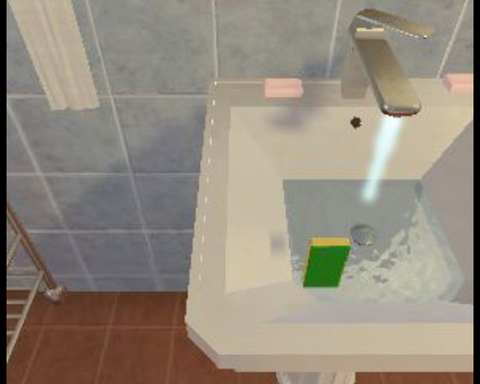
\includegraphics[width=2.660cm,height=2.128cm]{figures/img/subject_tiles/alfred.png}}};
\draw[black!35,line width=0.35pt] (0.060,-1.290) rectangle (2.720,-3.418);
\node[anchor=north west,text=ACMDarkBlue,font=\scriptsize,inner sep=0] at (0.080,-3.438) {\href{https://arxiv.org/abs/1912.01734}{ALFRED}};
\node[anchor=north west,text=black!55,font=\tiny,inner sep=0] at (0.080,-3.668) {\href{https://arxiv.org/abs/1912.01734}{arXiv:1912.01734}};
\node[anchor=north west,inner sep=0] at (2.770,-1.290) {\href{https://arxiv.org/abs/2403.09227}{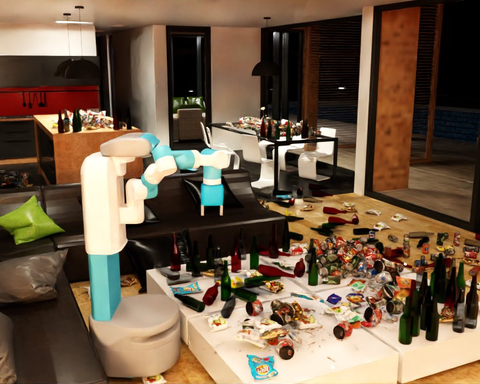
\includegraphics[width=2.660cm,height=2.128cm]{figures/img/subject_tiles/behavior1k.png}}};
\draw[black!35,line width=0.35pt] (2.770,-1.290) rectangle (5.430,-3.418);
\node[anchor=north west,text=ACMDarkBlue,font=\scriptsize,inner sep=0] at (2.790,-3.438) {\href{https://arxiv.org/abs/2403.09227}{BEHAVIOR-1K}};
\node[anchor=north west,text=black!55,font=\tiny,inner sep=0] at (2.790,-3.668) {\href{https://arxiv.org/abs/2403.09227}{arXiv:2403.09227}};
\node[anchor=north west,inner sep=0] at (5.480,-1.290) {\href{https://arxiv.org/abs/2112.03227}{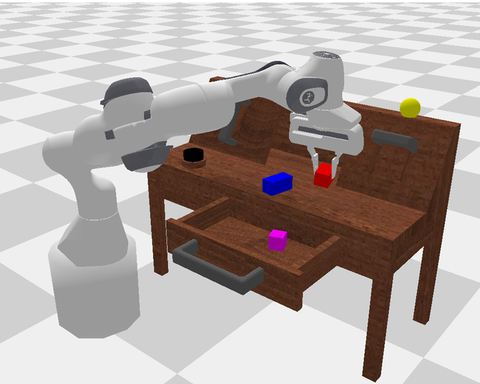
\includegraphics[width=2.660cm,height=2.128cm]{figures/img/subject_tiles/calvin.png}}};
\draw[black!35,line width=0.35pt] (5.480,-1.290) rectangle (8.140,-3.418);
\node[anchor=north west,text=ACMDarkBlue,font=\scriptsize,inner sep=0] at (5.500,-3.438) {\href{https://arxiv.org/abs/2112.03227}{CALVIN}};
\node[anchor=north west,text=black!55,font=\tiny,inner sep=0] at (5.500,-3.668) {\href{https://arxiv.org/abs/2112.03227}{arXiv:2112.03227}};
\node[anchor=north west,inner sep=0] at (8.190,-1.290) {\href{https://arxiv.org/abs/2410.01345}{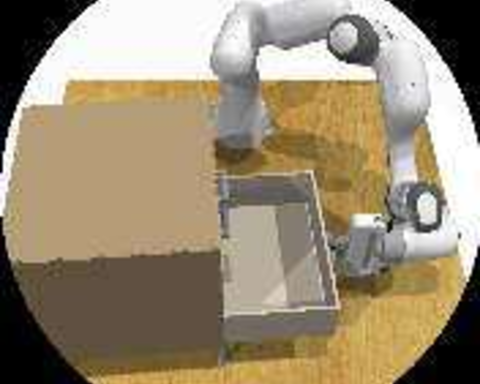
\includegraphics[width=2.660cm,height=2.128cm]{figures/img/subject_tiles/gembench.png}}};
\draw[black!35,line width=0.35pt] (8.190,-1.290) rectangle (10.850,-3.418);
\node[anchor=north west,text=ACMDarkBlue,font=\scriptsize,inner sep=0] at (8.210,-3.438) {\href{https://arxiv.org/abs/2410.01345}{GemBench}};
\node[anchor=north west,text=black!55,font=\tiny,inner sep=0] at (8.210,-3.668) {\href{https://arxiv.org/abs/2410.01345}{arXiv:2410.01345}};
\node[anchor=north west,inner sep=0] at (10.900,-1.290) {\href{https://arxiv.org/abs/2302.04659}{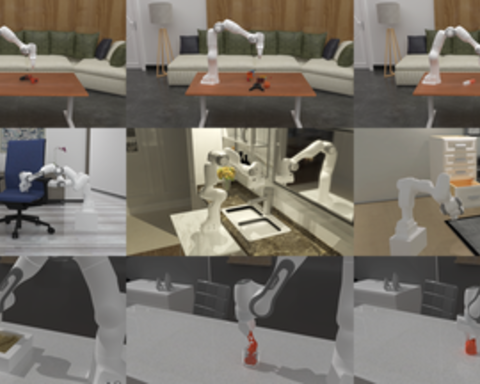
\includegraphics[width=2.660cm,height=2.128cm]{figures/img/subject_tiles/maniskill2.png}}};
\draw[black!35,line width=0.35pt] (10.900,-1.290) rectangle (13.560,-3.418);
\node[anchor=north west,text=ACMDarkBlue,font=\scriptsize,inner sep=0] at (10.920,-3.438) {\href{https://arxiv.org/abs/2302.04659}{ManiSkill2}};
\node[anchor=north west,text=black!55,font=\tiny,inner sep=0] at (10.920,-3.668) {\href{https://arxiv.org/abs/2302.04659}{arXiv:2302.04659}};
\node[anchor=north west,inner sep=0] at (0.060,-4.048) {\href{https://arxiv.org/abs/1910.10897}{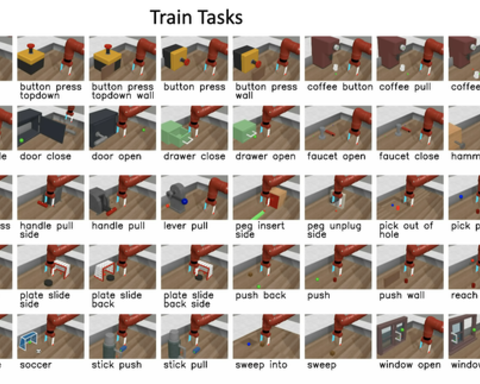
\includegraphics[width=2.660cm,height=2.128cm]{figures/img/subject_tiles/metaworld.png}}};
\draw[black!35,line width=0.35pt] (0.060,-4.048) rectangle (2.720,-6.176);
\node[anchor=north west,text=ACMDarkBlue,font=\scriptsize,inner sep=0] at (0.080,-6.196) {\href{https://arxiv.org/abs/1910.10897}{Meta-World}};
\node[anchor=north west,text=black!55,font=\tiny,inner sep=0] at (0.080,-6.426) {\href{https://arxiv.org/abs/1910.10897}{arXiv:1910.10897}};
\node[anchor=north west,inner sep=0] at (2.770,-4.048) {\href{https://arxiv.org/abs/2406.02523}{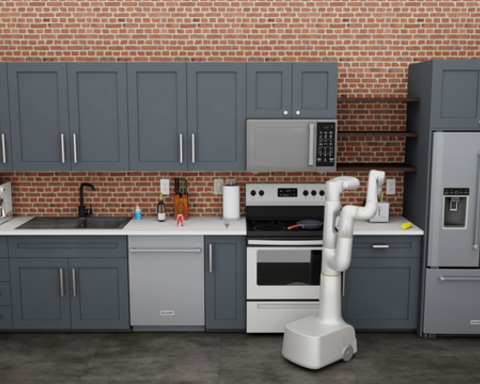
\includegraphics[width=2.660cm,height=2.128cm]{figures/img/subject_tiles/robocasa.png}}};
\draw[black!35,line width=0.35pt] (2.770,-4.048) rectangle (5.430,-6.176);
\node[anchor=north west,text=ACMDarkBlue,font=\scriptsize,inner sep=0] at (2.790,-6.196) {\href{https://arxiv.org/abs/2406.02523}{RoboCasa}};
\node[anchor=north west,text=black!55,font=\tiny,inner sep=0] at (2.790,-6.426) {\href{https://arxiv.org/abs/2406.02523}{arXiv:2406.02523}};
\node[anchor=north west,inner sep=0] at (5.480,-4.048) {\href{https://arxiv.org/abs/2306.03310}{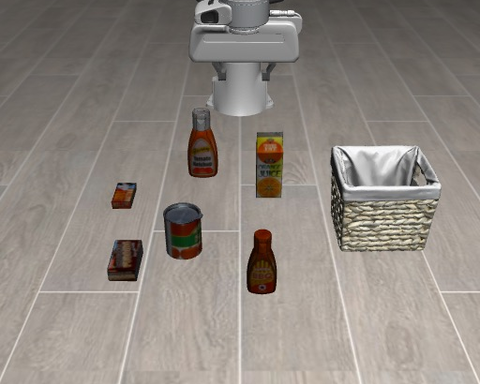
\includegraphics[width=2.660cm,height=2.128cm]{figures/img/subject_tiles/libero.png}}};
\draw[black!35,line width=0.35pt] (5.480,-4.048) rectangle (8.140,-6.176);
\node[anchor=north west,text=ACMDarkBlue,font=\scriptsize,inner sep=0] at (5.500,-6.196) {\href{https://arxiv.org/abs/2306.03310}{LIBERO}};
\node[anchor=north west,text=black!55,font=\tiny,inner sep=0] at (5.500,-6.426) {\href{https://arxiv.org/abs/2306.03310}{arXiv:2306.03310}};
\node[anchor=north west,inner sep=0] at (8.190,-4.048) {\href{https://arxiv.org/abs/2412.18194}{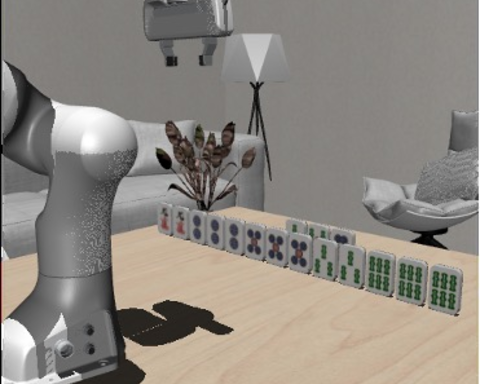
\includegraphics[width=2.660cm,height=2.128cm]{figures/img/subject_tiles/vlabench.png}}};
\draw[black!35,line width=0.35pt] (8.190,-4.048) rectangle (10.850,-6.176);
\node[anchor=north west,text=ACMDarkBlue,font=\scriptsize,inner sep=0] at (8.210,-6.196) {\href{https://arxiv.org/abs/2412.18194}{VLABench}};
\node[anchor=north west,text=black!55,font=\tiny,inner sep=0] at (8.210,-6.426) {\href{https://arxiv.org/abs/2412.18194}{arXiv:2412.18194}};
\node[anchor=north west,inner sep=0] at (10.900,-4.048) {\href{https://arxiv.org/abs/2310.13724}{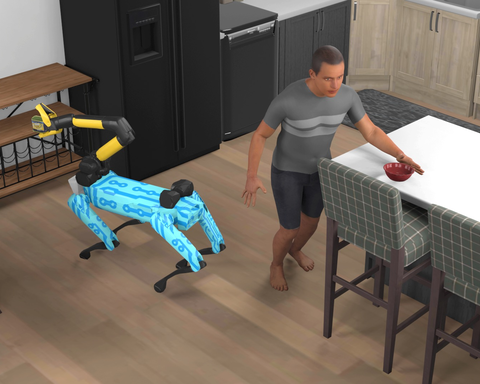
\includegraphics[width=2.660cm,height=2.128cm]{figures/img/subject_tiles/habitat30.png}}};
\draw[black!35,line width=0.35pt] (10.900,-4.048) rectangle (13.560,-6.176);
\node[anchor=north west,text=ACMDarkBlue,font=\scriptsize,inner sep=0] at (10.920,-6.196) {\href{https://arxiv.org/abs/2310.13724}{Habitat 3.0}};
\node[anchor=north west,text=black!55,font=\tiny,inner sep=0] at (10.920,-6.426) {\href{https://arxiv.org/abs/2310.13724}{arXiv:2310.13724}};
\fill[sgWM!78!black] (0,-6.906) rectangle (13.80,-7.406);
\node[anchor=west,text=white,font=\footnotesize\bfseries,inner sep=0] at (0.12,-7.156) {OPEN-LOOP world-model \& video-generation evaluation};
\node[anchor=north west,inner sep=0] at (0.060,-7.476) {\href{https://arxiv.org/abs/2410.15461}{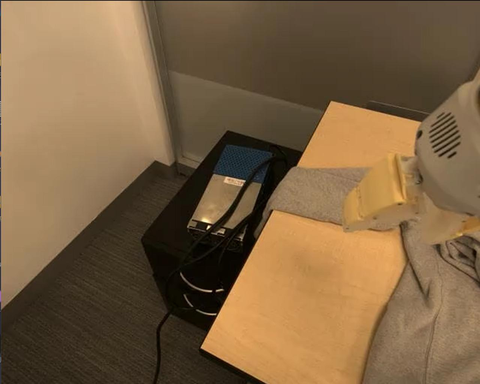
\includegraphics[width=2.660cm,height=2.128cm]{figures/img/subject_tiles/evabench.png}}};
\draw[black!35,line width=0.35pt] (0.060,-7.476) rectangle (2.720,-9.604);
\node[anchor=north west,text=ACMDarkBlue,font=\scriptsize,inner sep=0] at (0.080,-9.624) {\href{https://arxiv.org/abs/2410.15461}{EVA-Bench}};
\node[anchor=north west,text=black!55,font=\tiny,inner sep=0] at (0.080,-9.854) {\href{https://arxiv.org/abs/2410.15461}{arXiv:2410.15461}};
\node[anchor=north west,inner sep=0] at (2.770,-7.476) {\href{https://arxiv.org/abs/2505.09694}{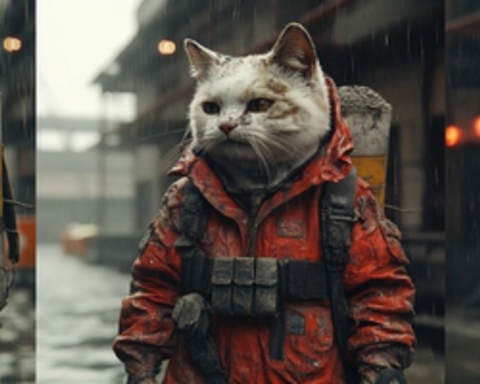
\includegraphics[width=2.660cm,height=2.128cm]{figures/img/subject_tiles/ewmbench.png}}};
\draw[black!35,line width=0.35pt] (2.770,-7.476) rectangle (5.430,-9.604);
\node[anchor=north west,text=ACMDarkBlue,font=\scriptsize,inner sep=0] at (2.790,-9.624) {\href{https://arxiv.org/abs/2505.09694}{EWMBench}};
\node[anchor=north west,text=black!55,font=\tiny,inner sep=0] at (2.790,-9.854) {\href{https://arxiv.org/abs/2505.09694}{arXiv:2505.09694}};
\node[anchor=north west,inner sep=0] at (5.480,-7.476) {\href{https://arxiv.org/abs/2501.09038}{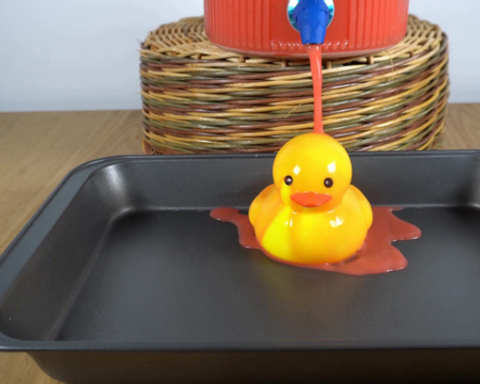
\includegraphics[width=2.660cm,height=2.128cm]{figures/img/subject_tiles/physicsiq.png}}};
\draw[black!35,line width=0.35pt] (5.480,-7.476) rectangle (8.140,-9.604);
\node[anchor=north west,text=ACMDarkBlue,font=\scriptsize,inner sep=0] at (5.500,-9.624) {\href{https://arxiv.org/abs/2501.09038}{Physics-IQ}};
\node[anchor=north west,text=black!55,font=\tiny,inner sep=0] at (5.500,-9.854) {\href{https://arxiv.org/abs/2501.09038}{arXiv:2501.09038}};
\node[anchor=north west,inner sep=0] at (8.190,-7.476) {\href{https://arxiv.org/abs/2106.08261}{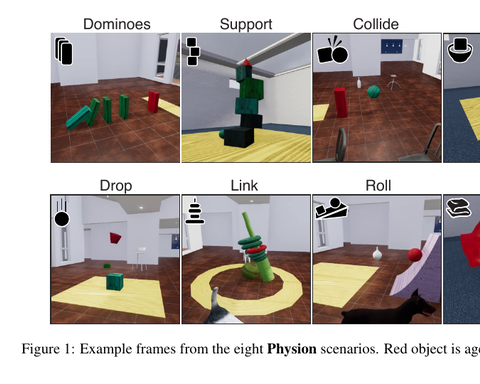
\includegraphics[width=2.660cm,height=2.128cm]{figures/img/subject_tiles/physion.png}}};
\draw[black!35,line width=0.35pt] (8.190,-7.476) rectangle (10.850,-9.604);
\node[anchor=north west,text=ACMDarkBlue,font=\scriptsize,inner sep=0] at (8.210,-9.624) {\href{https://arxiv.org/abs/2106.08261}{Physion}};
\node[anchor=north west,text=black!55,font=\tiny,inner sep=0] at (8.210,-9.854) {\href{https://arxiv.org/abs/2106.08261}{arXiv:2106.08261}};
\node[anchor=north west,inner sep=0] at (10.900,-7.476) {\href{https://arxiv.org/abs/2306.15668}{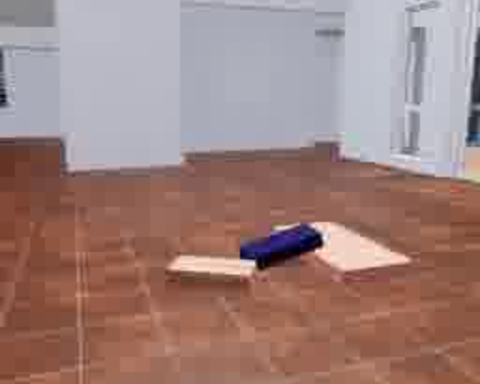
\includegraphics[width=2.660cm,height=2.128cm]{figures/img/subject_tiles/physionpp.png}}};
\draw[black!35,line width=0.35pt] (10.900,-7.476) rectangle (13.560,-9.604);
\node[anchor=north west,text=ACMDarkBlue,font=\scriptsize,inner sep=0] at (10.920,-9.624) {\href{https://arxiv.org/abs/2306.15668}{Physion++}};
\node[anchor=north west,text=black!55,font=\tiny,inner sep=0] at (10.920,-9.854) {\href{https://arxiv.org/abs/2306.15668}{arXiv:2306.15668}};
\node[anchor=north west,inner sep=0] at (0.060,-10.234) {\href{https://arxiv.org/abs/2406.03520}{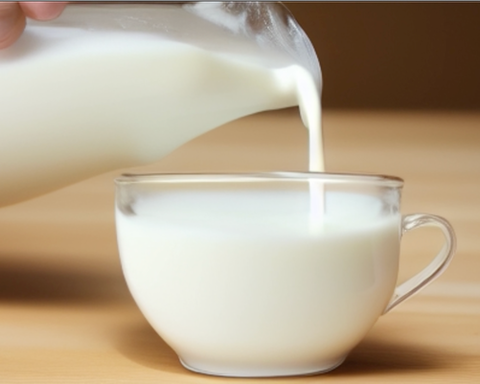
\includegraphics[width=2.660cm,height=2.128cm]{figures/img/subject_tiles/videophy.png}}};
\draw[black!35,line width=0.35pt] (0.060,-10.234) rectangle (2.720,-12.362);
\node[anchor=north west,text=ACMDarkBlue,font=\scriptsize,inner sep=0] at (0.080,-12.382) {\href{https://arxiv.org/abs/2406.03520}{VideoPhy}};
\node[anchor=north west,text=black!55,font=\tiny,inner sep=0] at (0.080,-12.612) {\href{https://arxiv.org/abs/2406.03520}{arXiv:2406.03520}};
\node[anchor=north west,inner sep=0] at (2.770,-10.234) {\href{https://arxiv.org/abs/2502.20694}{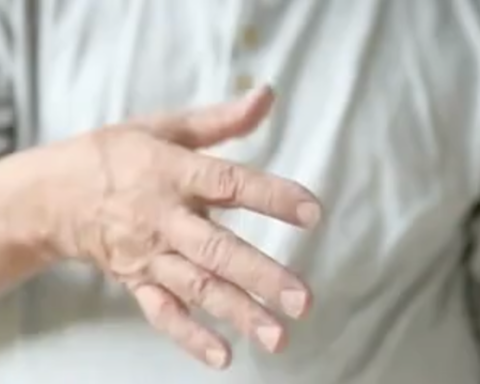
\includegraphics[width=2.660cm,height=2.128cm]{figures/img/subject_tiles/worldmodelbench.png}}};
\draw[black!35,line width=0.35pt] (2.770,-10.234) rectangle (5.430,-12.362);
\node[anchor=north west,text=ACMDarkBlue,font=\scriptsize,inner sep=0] at (2.790,-12.382) {\href{https://arxiv.org/abs/2502.20694}{WorldModelBench}};
\node[anchor=north west,text=black!55,font=\tiny,inner sep=0] at (2.790,-12.612) {\href{https://arxiv.org/abs/2502.20694}{arXiv:2502.20694}};
\node[anchor=north west,inner sep=0] at (5.480,-10.234) {\href{https://arxiv.org/abs/2504.00983}{
\includegraphics[width=2.660cm,height=2.128cm]{figures/img/subject_tiles/worldscore.png}}};
\draw[black!35,line width=0.35pt] (5.480,-10.234) rectangle (8.140,-12.362);
\node[anchor=north west,text=ACMDarkBlue,font=\scriptsize,inner sep=0] at (5.500,-12.382) {\href{https://arxiv.org/abs/2504.00983}{WorldScore}};
\node[anchor=north west,text=black!55,font=\tiny,inner sep=0] at (5.500,-12.612) {\href{https://arxiv.org/abs/2504.00983}{arXiv:2504.00983}};
\node[anchor=north west,inner sep=0] at (8.190,-10.234) {\href{https://arxiv.org/abs/2503.21755}{
\includegraphics[width=2.660cm,height=2.128cm]{figures/img/subject_tiles/vbench20.png}}};
\draw[black!35,line width=0.35pt] (8.190,-10.234) rectangle (10.850,-12.362);
\node[anchor=north west,text=ACMDarkBlue,font=\scriptsize,inner sep=0] at (8.210,-12.382) {\href{https://arxiv.org/abs/2503.21755}{VBench-2.0}};
\node[anchor=north west,text=black!55,font=\tiny,inner sep=0] at (8.210,-12.612) {\href{https://arxiv.org/abs/2503.21755}{arXiv:2503.21755}};
\node[anchor=north west,inner sep=0] at (10.900,-10.234) {\href{https://arxiv.org/abs/2506.04363}{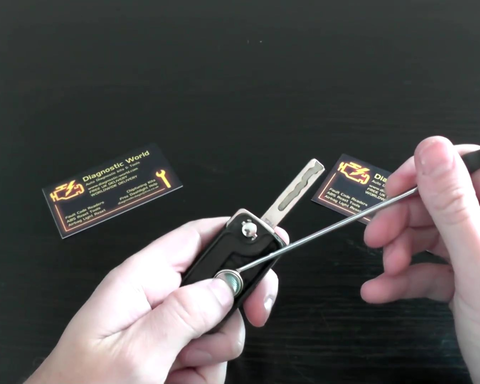
\includegraphics[width=2.660cm,height=2.128cm]{figures/img/subject_tiles/worldprediction.png}}};
\draw[black!35,line width=0.35pt] (10.900,-10.234) rectangle (13.560,-12.362);
\node[anchor=north west,text=ACMDarkBlue,font=\scriptsize,inner sep=0] at (10.920,-12.382) {\href{https://arxiv.org/abs/2506.04363}{WorldPrediction}};
\node[anchor=north west,text=black!55,font=\tiny,inner sep=0] at (10.920,-12.612) {\href{https://arxiv.org/abs/2506.04363}{arXiv:2506.04363}};
\fill[sgBridge!78!black] (0,-13.092) rectangle (13.80,-13.592);
\node[anchor=west,text=white,font=\footnotesize\bfseries,inner sep=0] at (0.12,-13.342) {PREDICTION-TO-ACTION bridges};
\node[anchor=north west,inner sep=0] at (0.060,-13.662) {\href{https://arxiv.org/abs/2410.18072}{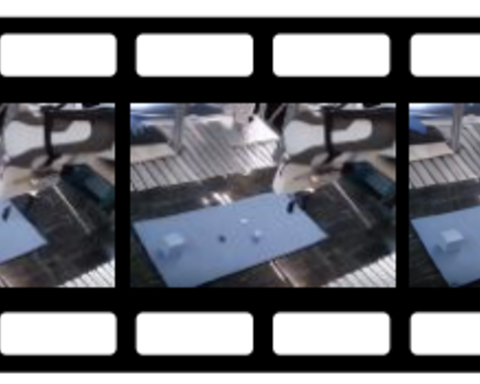
\includegraphics[width=2.660cm,height=2.128cm]{figures/img/subject_tiles/worldsimbench.png}}};
\draw[black!35,line width=0.35pt] (0.060,-13.662) rectangle (2.720,-15.790);
\node[anchor=north west,text=ACMDarkBlue,font=\scriptsize,inner sep=0] at (0.080,-15.810) {\href{https://arxiv.org/abs/2410.18072}{WorldSimBench}};
\node[anchor=north west,text=black!55,font=\tiny,inner sep=0] at (0.080,-16.040) {\href{https://arxiv.org/abs/2410.18072}{arXiv:2410.18072}};
\node[anchor=north west,inner sep=0] at (2.770,-13.662) {\href{https://arxiv.org/abs/2510.18135}{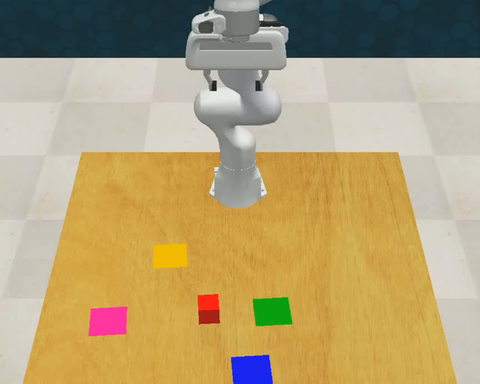
\includegraphics[width=2.660cm,height=2.128cm]{figures/img/subject_tiles/worldinworld.png}}};
\draw[black!35,line width=0.35pt] (2.770,-13.662) rectangle (5.430,-15.790);
\node[anchor=north west,text=ACMDarkBlue,font=\scriptsize,inner sep=0] at (2.790,-15.810) {\href{https://arxiv.org/abs/2510.18135}{World-in-World}};
\node[anchor=north west,text=black!55,font=\tiny,inner sep=0] at (2.790,-16.040) {\href{https://arxiv.org/abs/2510.18135}{arXiv:2510.18135}};
\node[anchor=north west,inner sep=0] at (5.480,-13.662) {\href{https://arxiv.org/abs/2604.19092}{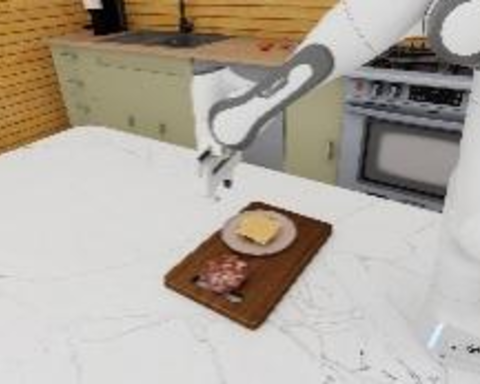
\includegraphics[width=2.660cm,height=2.128cm]{figures/img/subject_tiles/robowmbench.png}}};
\draw[black!35,line width=0.35pt] (5.480,-13.662) rectangle (8.140,-15.790);
\node[anchor=north west,text=ACMDarkBlue,font=\scriptsize,inner sep=0] at (5.500,-15.810) {\href{https://arxiv.org/abs/2604.19092}{RoboWM-Bench}};
\node[anchor=north west,text=black!55,font=\tiny,inner sep=0] at (5.500,-16.040) {\href{https://arxiv.org/abs/2604.19092}{arXiv:2604.19092}};
\node[anchor=north west,inner sep=0] at (8.190,-13.662) {\href{https://arxiv.org/abs/2602.08971}{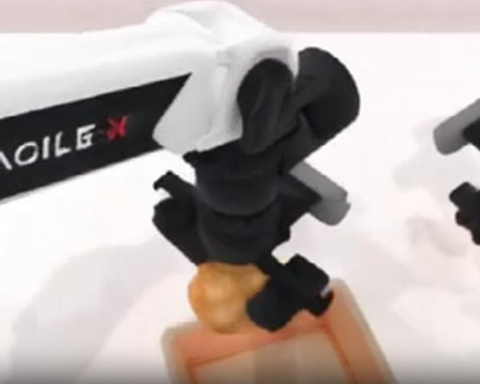
\includegraphics[width=2.660cm,height=2.128cm]{figures/img/subject_tiles/worldarena.png}}};
\draw[black!35,line width=0.35pt] (8.190,-13.662) rectangle (10.850,-15.790);
\node[anchor=north west,text=ACMDarkBlue,font=\scriptsize,inner sep=0] at (8.210,-15.810) {\href{https://arxiv.org/abs/2602.08971}{WorldArena}};
\node[anchor=north west,text=black!55,font=\tiny,inner sep=0] at (8.210,-16.040) {\href{https://arxiv.org/abs/2602.08971}{arXiv:2602.08971}};
\end{tikzpicture}}
\caption{\textbf{Benchmarks across the surveyed corpus.} Representative subject figures from the catalogue, grouped by evaluation lane rather than embodiment: \emph{closed-loop} task-success suites, \emph{open-loop} world-model and video-generation evaluation, and the \emph{prediction-to-action bridges}. Each panel is a live hyperlink to the source paper on arXiv and is annotated with its arXiv id (per-panel figure provenance in Table~\ref{tab:panel_provenance}); the figure is vector with photographs embedded at full resolution, so it can be zoomed without pixelation. Only figures that depict the benchmark's task or scene are shown; results and leaderboard figures appear in Figure~\ref{fig:results_gallery}. Benchmarks with no locatable subject figure are omitted, not fabricated. Images \textcopyright\ their respective authors, reproduced for scholarly review.}
\Description{A gallery of benchmark subject figures in three lane bands. The top band, closed-loop task-success suites, shows ten policy and embodied benchmark scenes (robot arms and simulated households). The middle band, open-loop world-model and video-generation evaluation, shows ten generated-video or physical-scene samples. The bottom band, prediction-to-action bridges, shows four world-model benchmark scenes. Each panel is labelled with the benchmark name and its arXiv id.}
\label{fig:subject_gallery}
\end{figure*}


\subsection{Policy suites}
\label{sec:lane_policy}

The policy lane (37 benchmarks) scores a policy by executing it and counting task success. Its
sub-families run from single- and dual-arm \emph{manipulation} (\S3.1.1: ARNOLD~\cite{arnold},
PerAct~\cite{peract}, FMB~\cite{fmb}, ManiSkill2~\cite{maniskill2}), through
\emph{generalization} suites that vary objects, scenes, and sim-to-real gaps (\S3.1.2:
LIBERO~\cite{libero}, THE COLOSSEUM~\cite{thecolosseum}, SIMPLER~\cite{simpler},
VIMA-Bench~\cite{vimabench}), to \emph{dexterous} hands (\S3.1.4: Bi-DexHands~\cite{bidexhands},
DexArt~\cite{dexart}, UniDexGrasp~\cite{unidexgrasp}). These suites are the backbone of policy
evaluation, and they are deliberately model-agnostic: they host whatever policy a user brings and are
careful not to privilege one architecture. That neutrality is exactly why they cannot, on their own,
answer whether a world-model policy beats a direct one. Table~\ref{tab:compare_capability} audits,
capability by capability, which benchmarks come closest to building such a contrast, and finds the
lane almost entirely agnostic.

% Per-capability deep-dive (P1 analog: Table 4/6): which benchmarks probe each capability cut,
% and whether each builds a VLA-vs-world-model contrast. Marks (Eval, VLA-vs-WM) are the catalogue's
% own values (docs/assets/catalog_p3.js); native contrasts cluster in the reasoning cuts.
{\footnotesize
\setlength{\tabcolsep}{5pt}
\renewcommand{\arraystretch}{1.08}
\begin{longtable}{@{}p{0.26\textwidth} c c >{\raggedright\arraybackslash}p{0.48\textwidth} c@{}}
\caption{\textbf{Capability deep-dive}: the benchmarks that probe each of the $\beta$ capability
cuts, and whether each builds a native VLA-vs-world-model contrast. Native contrasts cluster in the
hidden-state, theory-of-mind and counterfactual \emph{reasoning} cuts (LIBERO-Mem, ComPhy, AGENT,
BIB, ACRE, CoPhy, CausalWorld); the long-horizon and social \emph{task-success} cuts are largely
model-agnostic (ALFWorld's abstract-to-grounded transfer is the lone partial). \textbf{Eval}: \dopen/\dclosed. \textbf{VLA vs WM}: \yy\ native contrast,
\pp\ partial, \dm\ model-agnostic; each cut's header tallies the fraction of its benchmarks that
build any (native or partial) contrast.}\label{tab:compare_capability}\\
\toprule
\textbf{Benchmark} & \textbf{Year} & \textbf{Eval} & \textbf{What it probes} & \textbf{VLA vs WM}\\
\midrule
\endfirsthead
\multicolumn{5}{@{}l}{\footnotesize\emph{Table~\ref{tab:compare_capability} (continued)}}\\
\toprule
\textbf{Benchmark} & \textbf{Year} & \textbf{Eval} & \textbf{What it probes} & \textbf{VLA vs WM}\\
\midrule
\endhead
\bottomrule
\endlastfoot
\multicolumn{4}{@{}l}{\rule{0pt}{2.2ex}\textbf{\textsf{Hidden-state / memory / occlusion}}} & {\footnotesize\itshape 3/4}\\[1pt]
\textbf{LIBERO-Mem}~\cite{liberomem} & 2025 & \dclosed & occluded object state carried across time & \yy\\
\textbf{TEACh}~\cite{teach} & 2021 & \dclosed & partner belief and history via dialog & \dm\\
\textbf{ComPhy}~\cite{comphy} & 2022 & \dopen & hidden mass and charge inferred from collisions & \yy\\
\textbf{Bongard-HOI}~\cite{bongardhoi} & 2022 & \dopen & few-shot hidden-concept induction & \pp\\
\midrule
\multicolumn{4}{@{}l}{\rule{0pt}{2.2ex}\textbf{\textsf{Theory-of-mind}}} & {\footnotesize\itshape 3/4}\\[1pt]
\textbf{AGENT}~\cite{agent} & 2021 & \dopen & expectations over an agent's goals and actions & \yy\\
\textbf{BIB}~\cite{bib} & 2021 & \dopen & infant-style goal inference from behaviour & \yy\\
\textbf{PHASE}~\cite{phase} & 2021 & \dclosed & social relations and goals inferred from motion & \pp\\
\textbf{SocialAI}~\cite{socialai} & 2021 & \dclosed & language-based social interaction with agents & \dm\\
\midrule
\multicolumn{4}{@{}l}{\rule{0pt}{2.2ex}\textbf{\textsf{Counterfactual / physical inference}}} & {\footnotesize\itshape 3/6}\\[1pt]
\textbf{WorldPrediction}~\cite{worldprediction} & 2025 & \dopen & discriminate correct vs counterfactual action & \dm\\
\textbf{Physion}~\cite{physion} & 2021 & \dopen & predict a physical outcome from vision & \dm\\
\textbf{Physion++}~\cite{physionpp} & 2023 & \dopen & infer latent physical properties online & \dm\\
\textbf{ACRE}~\cite{acre} & 2021 & \dopen & abstract causal reasoning over blicket tests & \yy\\
\textbf{CoPhy}~\cite{cophy} & 2019 & \dopen & counterfactual outcome under a changed cause & \yy\\
\textbf{CausalWorld}~\cite{causalworld} & 2020 & \dclosed & causal do-interventions on task variables & \yy\\
\midrule
\multicolumn{4}{@{}l}{\rule{0pt}{2.2ex}\textbf{\textsf{Long-horizon / compositional}}} & {\footnotesize\itshape 1/6}\\[1pt]
\textbf{CALVIN}~\cite{calvin} & 2021 & \dclosed & chain several language subtasks in a row & \dm\\
\textbf{BEHAVIOR-1K}~\cite{behavior1k} & 2024 & \dclosed & 1000 long-horizon household activities & \dm\\
\textbf{ALFRED}~\cite{alfred} & 2019 & \dclosed & instruction to action under partial view & \dm\\
\textbf{ALFWorld}~\cite{alfworld} & 2020 & \dclosed & abstract-text to grounded-task transfer & \pp\\
\textbf{EmbodiedBench}~\cite{embodiedbench} & 2025 & \dclosed & broad long-horizon embodied planning & \dm\\
\textbf{PARTNR}~\cite{partnr} & 2024 & \dclosed & human-robot collaborative household tasks & \dm\\
\midrule
\multicolumn{4}{@{}l}{\rule{0pt}{2.2ex}\textbf{\textsf{Social / multi-agent}}} & {\footnotesize\itshape 0/5}\\[1pt]
\textbf{Habitat 3.0}~\cite{habitat30} & 2023 & \dclosed & human-robot co-habitation and hand-off & \dm\\
\textbf{SocNavBench}~\cite{socnavbench} & 2021 & \dclosed & socially compliant navigation & \dm\\
\textbf{Melting Pot}~\cite{meltingpot} & 2021 & \dclosed & mixed-motive multi-agent generalization & \dm\\
\textbf{SMAC}~\cite{smac} & 2019 & \dclosed & cooperative multi-agent micro-control & \dm\\
\textbf{CrowdNav}~\cite{crowdnav} & 2018 & \dclosed & socially-aware navigation among pedestrians & \dm\\
\end{longtable}
}


\subsection{Embodied agents}
\label{sec:lane_embodied}

The embodied-agent lane is the largest (85 benchmarks) and the most diverse. It spans
\emph{long-horizon} household and planning tasks (\S3.2.1: ALFRED~\cite{alfred},
BEHAVIOR-1K~\cite{behavior1k}, EmbodiedBench~\cite{embodiedbench}), \emph{social and multi-agent}
settings (\S3.2.2: Habitat~3.0~\cite{habitat30}, Overcooked-AI~\cite{overcookedai},
Melting~Pot~\cite{meltingpot}), \emph{navigation} (\S3.2.3: Habitat~\cite{habitat},
HM3D~\cite{hm3d}, GOAT-Bench~\cite{goatbench}), \emph{autonomous driving} (\S3.2.4:
CARLA~\cite{carla}, Bench2Drive~\cite{bench2drive}, Waymax~\cite{waymax}), \emph{counterfactual}
reasoning (\S3.2.5: CausalWorld~\cite{causalworld}, CoPhy~\cite{cophy}, ACRE~\cite{acre}), and
\emph{locomotion} (\S3.2.6: HumanoidBench~\cite{humanoidbench}, Barkour~\cite{barkour},
Isaac~Gym~\cite{isaacgym}). Two observations matter for the survey's question. First, like the policy
lane, these suites are overwhelmingly model-agnostic. Second, the counterfactual sub-family, which
is where predictive world modelling should most plausibly help, is the thinnest: it is populated by
causal-reasoning tasks but almost never run as a closed-loop VLA-versus-world-model contrast.

\subsection{World-model evaluation}
\label{sec:lane_wmeval}

The world-model-evaluation lane (34 benchmarks) scores prediction and generation directly, with no
action taken. Its sub-families are \emph{generation quality} (\S3.3.1: VBench~\cite{vbench},
EvalCrafter~\cite{evalcrafter}, EWMBench~\cite{ewmbench}, EVA-Bench~\cite{evabench}),
\emph{physical reasoning} (\S3.3.2: IntPhys~\cite{intphys}, PhysBench~\cite{physbench},
PhyGenBench~\cite{phygenbench}, Physics-IQ~\cite{physicsiq}), \emph{counterfactual} video reasoning
(\S3.3.3: CLEVRER~\cite{clevrer}, WorldPrediction~\cite{worldprediction}), and a driving world model
(\S3.3.4: Vista~\cite{vista}). Table~\ref{tab:compare_wmeval} is a deep-dive over all 34: it records
what each scores (generation, question-answering, or prediction), the signal it uses (automatic
metric, accuracy, violation-of-expectation, or human rating), and whether it touches physical
grounding. The lane's defining limitation is uniform: every benchmark scores open-loop, and none
executes what it predicts, so a high generation score certifies visual quality but says nothing about
task success.

% World-model-evaluation lane deep-dive (P1 analog: Table 6, the skill-building branch deep-dive).
% The 34 wmeval-lane benchmarks by sub-type. Year + sub-type catalogue-grounded; Mode + Signal are
% colour-coded categoricals (mirroring P1 table6's Form/Domain), Physical = physical-law grounding.
{\footnotesize
\setlength{\tabcolsep}{5pt}
\renewcommand{\arraystretch}{1.0}
% colour-coded categorical values (like p1_table6's Form/Domain)
\newcommand{\mgen}{\textcolor{teal!72!black}{\textsf{Gen}}}
\newcommand{\mqa}{\textcolor{blue!62!black}{\textsf{QA}}}
\newcommand{\mpred}{\textcolor{violet!72!black}{\textsf{Pred}}}
\newcommand{\sauto}{\textcolor{black!55}{\textsf{Auto}}}
\newcommand{\sacc}{\textcolor{ForestGreen!88!black}{\textsf{Acc}}}
\newcommand{\svoe}{\textcolor{orange!85!black}{\textsf{VOE}}}
\newcommand{\shuman}{\textcolor{magenta!72!black}{\textsf{Human}}}
\begin{longtable}{@{}p{0.25\textwidth} c c >{\raggedright\arraybackslash}p{0.40\textwidth} c c@{}}
\caption{\textbf{World-model-evaluation deep-dive}: the 34 benchmarks of the world-model-evaluation
lane, by sub-type -- the P3 counterpart of the skill-building branch deep-dive. \textbf{Mode}:
\mgen\ evaluates generated video, \mqa\ video question-answering, \mpred\ physical prediction.
\textbf{Signal}: \sauto\ computed/learned metric, \sacc\ accuracy vs ground truth, \svoe\
violation-of-expectation, \shuman\ human study. \textbf{Physical}: targets physical-law
understanding, \yy\ core, \pp\ adjacent, \nn\ general. Generation-quality suites dominate and are
physics-agnostic; only the physical-reasoning and physical-commonsense sub-types test physical law,
and every lane benchmark scores open-loop, never in a closed loop.}\label{tab:compare_wmeval}\\
\toprule
\textbf{Benchmark} & \textbf{Year} & \textbf{Mode} & \textbf{What it scores} & \textbf{Signal} & \textbf{Physical}\\
\midrule
\endfirsthead
\multicolumn{6}{@{}l}{\footnotesize\emph{Table~\ref{tab:compare_wmeval} (continued)}}\\
\toprule
\textbf{Benchmark} & \textbf{Year} & \textbf{Mode} & \textbf{What it scores} & \textbf{Signal} & \textbf{Physical}\\
\midrule
\endhead
\bottomrule
\endlastfoot
\multicolumn{6}{@{}l}{\rule{0pt}{2.0ex}\textbf{\textsf{Generation quality (multi-dimensional)}}}\\[1pt]
\textbf{EvalCrafter}~\cite{evalcrafter} & 2023 & \mgen & 17-metric text-to-video quality suite & \sauto & \nn\\
\textbf{FETV}~\cite{fetv} & 2023 & \mgen & fine-grained text-to-video quality & \sauto & \nn\\
\textbf{VBench}~\cite{vbench} & 2023 & \mgen & 16 disentangled generation dimensions & \sauto & \nn\\
\textbf{StoryBench}~\cite{storybench} & 2023 & \mgen & continuous story-visualisation quality & \sauto & \nn\\
\textbf{DEVIL}~\cite{devil} & 2024 & \mgen & content-dynamics quality of T2V & \sauto & \nn\\
\textbf{T2V-CompBench}~\cite{t2vcompbench} & 2024 & \mgen & compositional text-to-video quality & \sauto & \nn\\
\textbf{T2VScore}~\cite{t2vscore} & 2024 & \mgen & learned alignment + quality metric & \sauto & \nn\\
\textbf{TC-Bench}~\cite{tcbench} & 2024 & \mgen & temporal compositionality in generation & \sauto & \nn\\
\textbf{VideoScore}~\cite{videoscore} & 2024 & \mgen & learned automatic quality metric & \sauto & \nn\\
\textbf{EWMBench}~\cite{ewmbench} & 2025 & \mgen & scene / motion / semantic quality & \sauto & \nn\\
\textbf{VBench-2.0}~\cite{vbench20} & 2025 & \mgen & generation faithfulness & \sauto & \nn\\
\midrule
\multicolumn{6}{@{}l}{\rule{0pt}{2.0ex}\textbf{\textsf{Intuitive \& physical reasoning}}}\\[1pt]
\textbf{IntPhys}~\cite{intphys} & 2018 & \mpred & intuitive physics from video & \svoe & \yy\\
\textbf{Physion}~\cite{physion} & 2021 & \mpred & physical outcome prediction from vision & \sacc & \yy\\
\textbf{GRASP}~\cite{grasp} & 2023 & \mqa & intuitive physics in video MLLMs & \sacc & \yy\\
\textbf{Physion++}~\cite{physionpp} & 2023 & \mpred & prediction with online property inference & \sacc & \yy\\
\textbf{ContPhy}~\cite{contphy} & 2024 & \mqa & soft-body / fluid physical reasoning & \sacc & \yy\\
\textbf{Physics-IQ}~\cite{physicsiq} & 2025 & \mgen & physical realism of generated video & \sauto & \yy\\
\textbf{PhysBench}~\cite{physbench} & 2025 & \mqa & physical-world understanding for VLMs & \sacc & \yy\\
\textbf{PHYBench}~\cite{phybench} & 2025 & \mqa & physical perception and reasoning & \sacc & \yy\\
\textbf{IntPhys 2}~\cite{intphys2} & 2025 & \mpred & intuitive physics in complex scenes & \svoe & \yy\\
\midrule
\multicolumn{6}{@{}l}{\rule{0pt}{2.0ex}\textbf{\textsf{Physical commonsense in generated video}}}\\[1pt]
\textbf{PhyGenBench}~\cite{phygenbench} & 2024 & \mgen & physical-commonsense correctness in gen & \sauto & \yy\\
\textbf{VideoPhy}~\cite{videophy} & 2024 & \mgen & physical commonsense in generated video & \shuman & \yy\\
\textbf{VideoPhy-2}~\cite{videophy2} & 2025 & \mgen & action-centric physical commonsense & \shuman & \yy\\
\textbf{PhyWorldBench}~\cite{phyworldbench} & 2025 & \mgen & physical realism in text-to-video & \shuman & \yy\\
\textbf{IPV-Bench}~\cite{ipvbench} & 2025 & \mgen & impossible-video generation + understanding & \sacc & \yy\\
\midrule
\multicolumn{6}{@{}l}{\rule{0pt}{2.0ex}\textbf{\textsf{Counterfactual / causal / temporal}}}\\[1pt]
\textbf{CATER}~\cite{cater} & 2019 & \mqa & compositional-action temporal reasoning & \sacc & \nn\\
\textbf{CLEVRER}~\cite{clevrer} & 2019 & \mqa & causal / counterfactual video reasoning & \sacc & \pp\\
\textbf{WorldPrediction}~\cite{worldprediction} & 2025 & \mqa & counterfactual action recognition & \sacc & \nn\\
\midrule
\multicolumn{6}{@{}l}{\rule{0pt}{2.0ex}\textbf{\textsf{Video-language alignment / hallucination}}}\\[1pt]
\textbf{VideoCon}~\cite{videocon} & 2023 & \mqa & robust video-language alignment & \sauto & \nn\\
\textbf{VideoHallucer}~\cite{videohallucer} & 2024 & \mqa & hallucination in video-language models & \sacc & \nn\\
\midrule
\multicolumn{6}{@{}l}{\rule{0pt}{2.0ex}\textbf{\textsf{World-model prediction \& world generation}}}\\[1pt]
\textbf{Vista}~\cite{vista} & 2024 & \mgen & driving world-model generation & \sauto & \pp\\
\textbf{EVA-Bench}~\cite{evabench} & 2024 & \mpred & embodied video anticipation & \sauto & \pp\\
\textbf{WorldModelBench}~\cite{worldmodelbench} & 2025 & \mgen & video world-model prediction quality & \shuman & \pp\\
\textbf{WorldScore}~\cite{worldscore} & 2025 & \mgen & controllable world-generation quality & \sauto & \nn\\
\end{longtable}
}

% RESULTS gallery (P1 analog: p1_fig9). AUTO-GENERATED by no_upload/gen_results_gallery_p3.py.
% Tiles are real results/leaderboard/metric plots cropped from each benchmark's arXiv paper;
% provenance in Table~\ref{tab:results_provenance}. Grouped by type of evidence.
\begin{figure*}[p]
\centering
\definecolor{rgA}{HTML}{1F618D}\definecolor{rgB}{HTML}{117A65}\definecolor{rgC}{HTML}{B9770E}%
\resizebox{\textwidth}{!}{%
\begin{tikzpicture}[x=1cm,y=1cm]
\fill[black!88] (0,0) rectangle (13.62,-0.72);
\node[anchor=west,text=white,font=\large\bfseries,inner sep=0] at (0.16,-0.36) {Results reported across the surveyed corpus};
\node[anchor=east,text=white!70,font=\scriptsize,inner sep=0] at (13.46,-0.36) {vector, zoomable, per-panel arXiv links};
\fill[rgA!82!black] (0,-0.720) rectangle (13.62,-1.220);
\node[anchor=west,text=white,font=\footnotesize\bfseries,inner sep=0] at (0.12,-0.970) {Leaderboard \& model-comparison charts};
\node[anchor=north west,inner sep=0] at (0.060,-1.290) {\href{https://arxiv.org/abs/2510.18135}{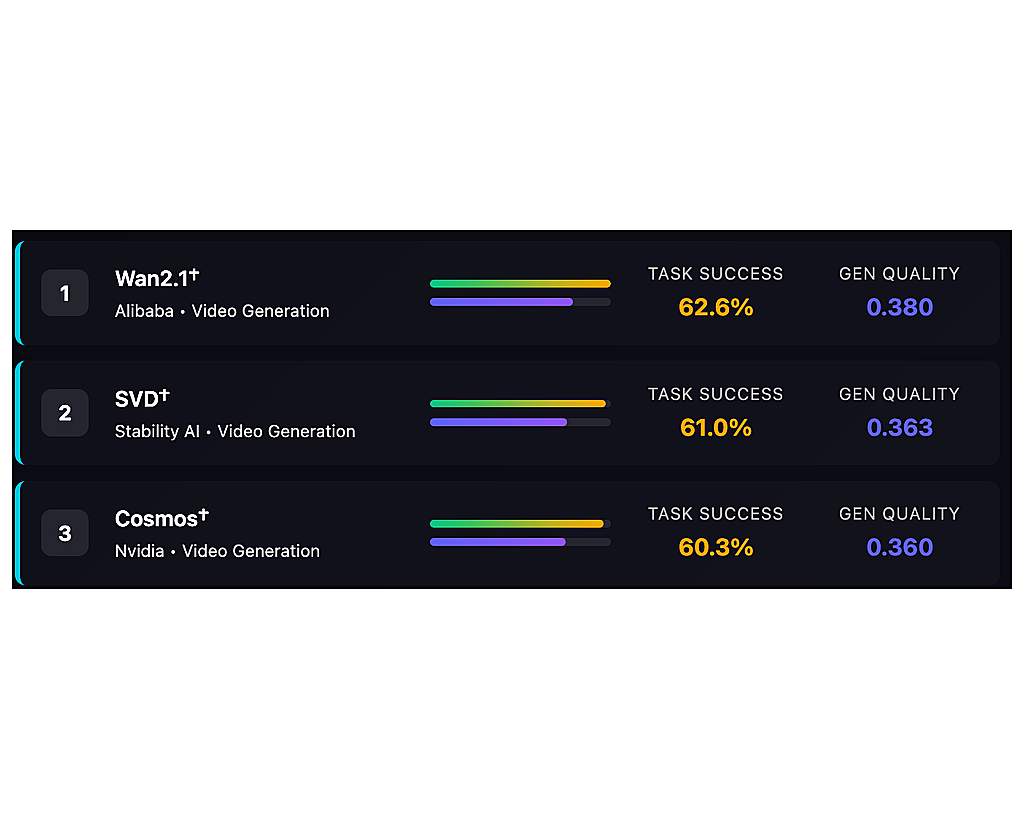
\includegraphics[width=3.300cm,height=2.640cm]{figures/img/results_tiles/worldinworld.png}}};
\draw[black!35,line width=0.35pt] (0.060,-1.290) rectangle (3.360,-3.930);
\node[anchor=north west,text=ACMDarkBlue,font=\scriptsize,inner sep=0] at (0.080,-3.950) {\href{https://arxiv.org/abs/2510.18135}{World-in-World}};
\node[anchor=north west,text=black!55,font=\tiny,inner sep=0] at (0.080,-4.180) {\href{https://arxiv.org/abs/2510.18135}{arXiv:2510.18135}};
\node[anchor=north west,inner sep=0] at (3.420,-1.290) {\href{https://arxiv.org/abs/2310.11440}{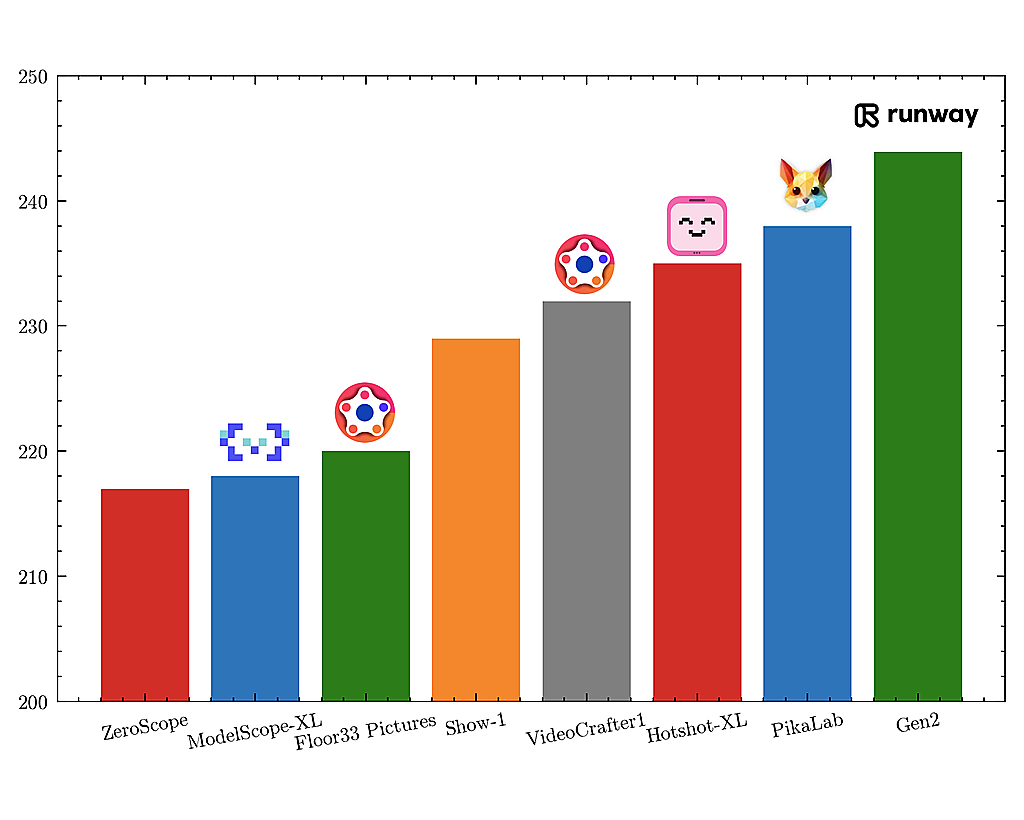
\includegraphics[width=3.300cm,height=2.640cm]{figures/img/results_tiles/evalcrafter_bars.png}}};
\draw[black!35,line width=0.35pt] (3.420,-1.290) rectangle (6.720,-3.930);
\node[anchor=north west,text=ACMDarkBlue,font=\scriptsize,inner sep=0] at (3.440,-3.950) {\href{https://arxiv.org/abs/2310.11440}{EvalCrafter}};
\node[anchor=north west,text=black!55,font=\tiny,inner sep=0] at (3.440,-4.180) {\href{https://arxiv.org/abs/2310.11440}{arXiv:2310.11440}};
\node[anchor=north west,inner sep=0] at (6.780,-1.290) {\href{https://arxiv.org/abs/2406.15252}{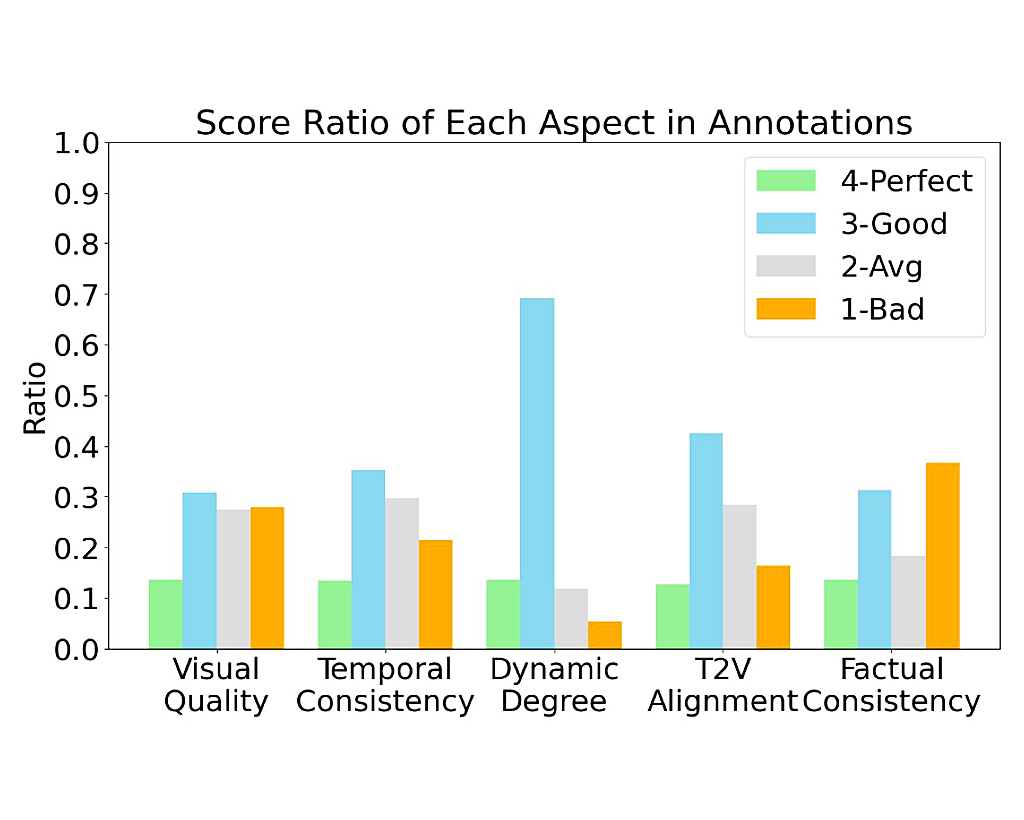
\includegraphics[width=3.300cm,height=2.640cm]{figures/img/results_tiles/videoscore.png}}};
\draw[black!35,line width=0.35pt] (6.780,-1.290) rectangle (10.080,-3.930);
\node[anchor=north west,text=ACMDarkBlue,font=\scriptsize,inner sep=0] at (6.800,-3.950) {\href{https://arxiv.org/abs/2406.15252}{VideoScore}};
\node[anchor=north west,text=black!55,font=\tiny,inner sep=0] at (6.800,-4.180) {\href{https://arxiv.org/abs/2406.15252}{arXiv:2406.15252}};
\node[anchor=north west,inner sep=0] at (10.140,-1.290) {\href{https://arxiv.org/abs/2502.20694}{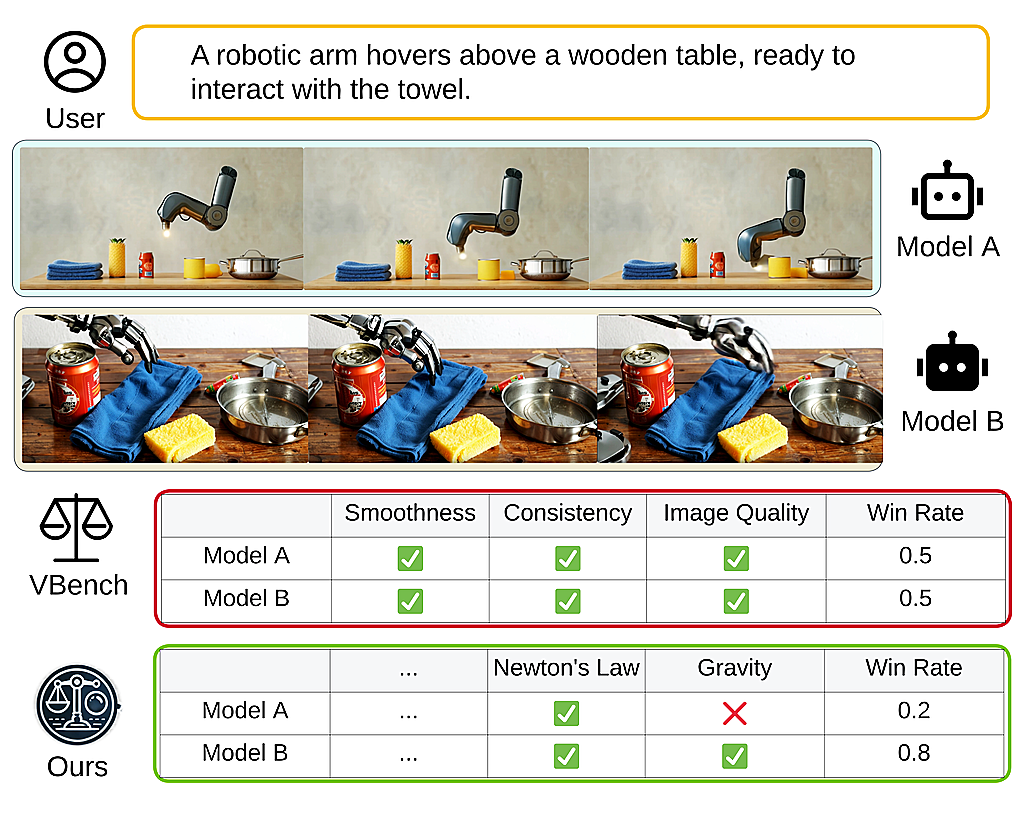
\includegraphics[width=3.300cm,height=2.640cm]{figures/img/results_tiles/worldmodelbench.png}}};
\draw[black!35,line width=0.35pt] (10.140,-1.290) rectangle (13.440,-3.930);
\node[anchor=north west,text=ACMDarkBlue,font=\scriptsize,inner sep=0] at (10.160,-3.950) {\href{https://arxiv.org/abs/2502.20694}{WorldModelBench}};
\node[anchor=north west,text=black!55,font=\tiny,inner sep=0] at (10.160,-4.180) {\href{https://arxiv.org/abs/2502.20694}{arXiv:2502.20694}};
\fill[rgB!82!black] (0,-4.690) rectangle (13.62,-5.190);
\node[anchor=west,text=white,font=\footnotesize\bfseries,inner sep=0] at (0.12,-4.940) {Per-dimension radar \& multi-metric};
\node[anchor=north west,inner sep=0] at (0.060,-5.260) {\href{https://arxiv.org/abs/2311.17982}{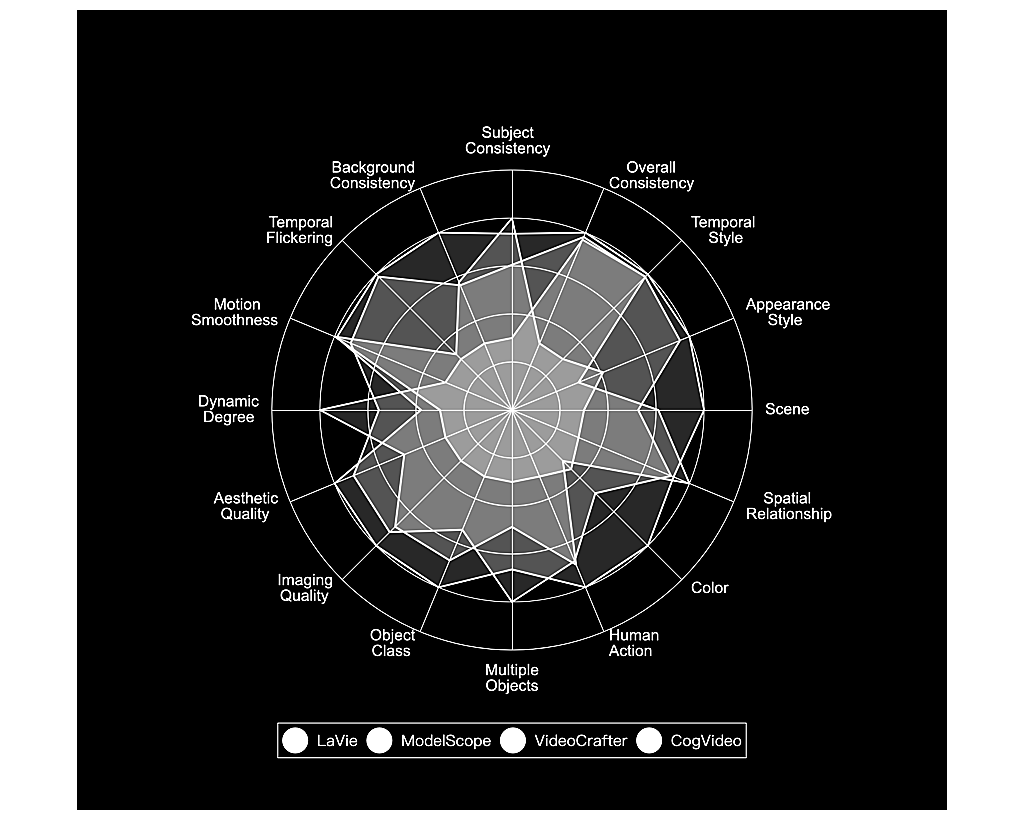
\includegraphics[width=3.300cm,height=2.640cm]{figures/img/results_tiles/vbench_radar.png}}};
\draw[black!35,line width=0.35pt] (0.060,-5.260) rectangle (3.360,-7.900);
\node[anchor=north west,text=ACMDarkBlue,font=\scriptsize,inner sep=0] at (0.080,-7.920) {\href{https://arxiv.org/abs/2311.17982}{VBench}};
\node[anchor=north west,text=black!55,font=\tiny,inner sep=0] at (0.080,-8.150) {\href{https://arxiv.org/abs/2311.17982}{arXiv:2311.17982}};
\node[anchor=north west,inner sep=0] at (3.420,-5.260) {\href{https://arxiv.org/abs/2505.09694}{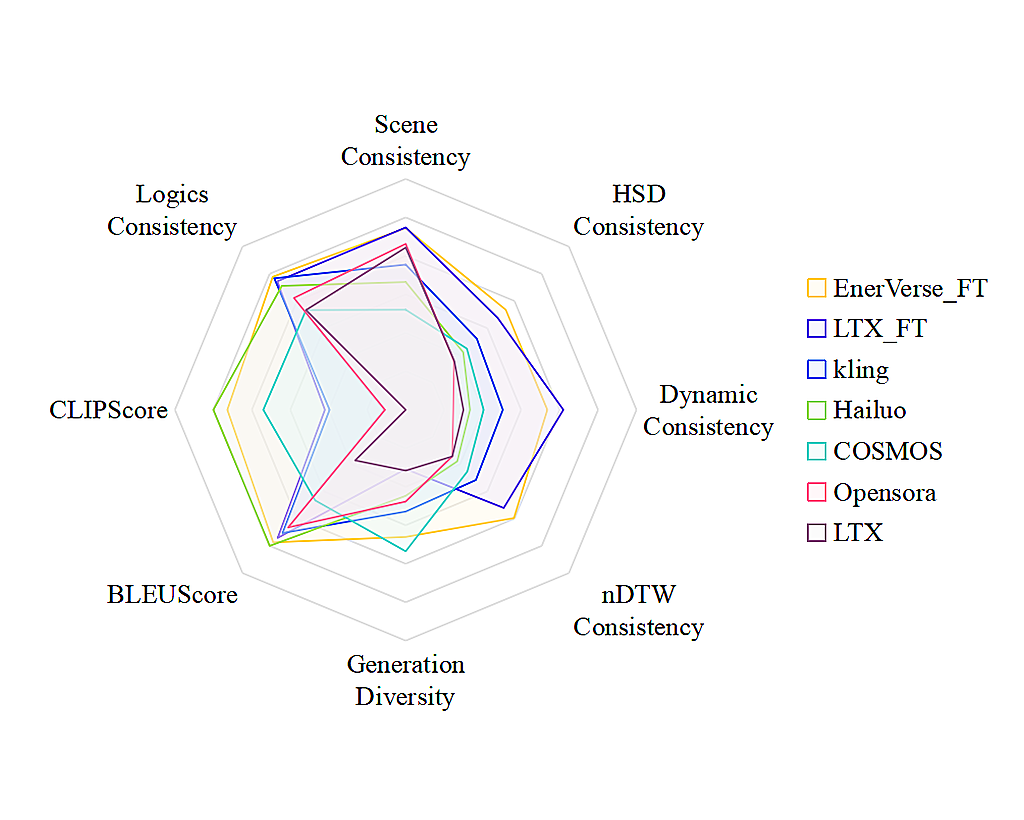
\includegraphics[width=3.300cm,height=2.640cm]{figures/img/results_tiles/ewmbench.png}}};
\draw[black!35,line width=0.35pt] (3.420,-5.260) rectangle (6.720,-7.900);
\node[anchor=north west,text=ACMDarkBlue,font=\scriptsize,inner sep=0] at (3.440,-7.920) {\href{https://arxiv.org/abs/2505.09694}{EWMBench}};
\node[anchor=north west,text=black!55,font=\tiny,inner sep=0] at (3.440,-8.150) {\href{https://arxiv.org/abs/2505.09694}{arXiv:2505.09694}};
\node[anchor=north west,inner sep=0] at (6.780,-5.260) {\href{https://arxiv.org/abs/2602.08971}{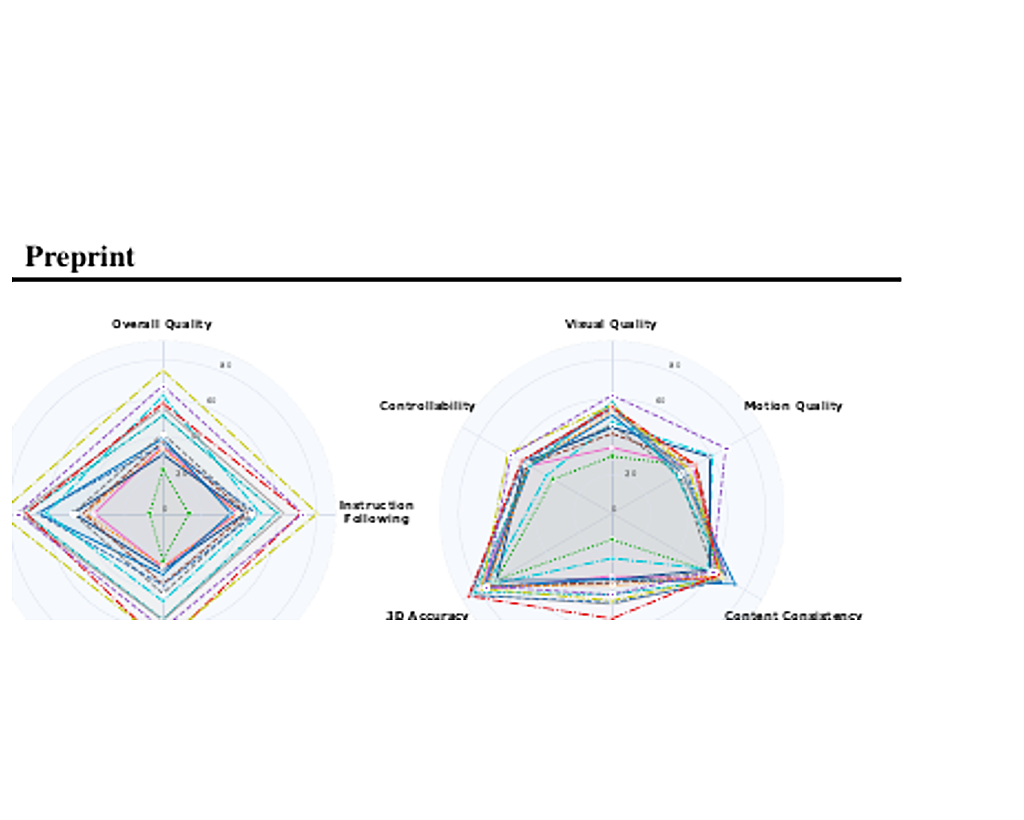
\includegraphics[width=3.300cm,height=2.640cm]{figures/img/results_tiles/worldarena.png}}};
\draw[black!35,line width=0.35pt] (6.780,-5.260) rectangle (10.080,-7.900);
\node[anchor=north west,text=ACMDarkBlue,font=\scriptsize,inner sep=0] at (6.800,-7.920) {\href{https://arxiv.org/abs/2602.08971}{WorldArena}};
\node[anchor=north west,text=black!55,font=\tiny,inner sep=0] at (6.800,-8.150) {\href{https://arxiv.org/abs/2602.08971}{arXiv:2602.08971}};
\node[anchor=north west,inner sep=0] at (10.140,-5.260) {\href{https://arxiv.org/abs/2310.11440}{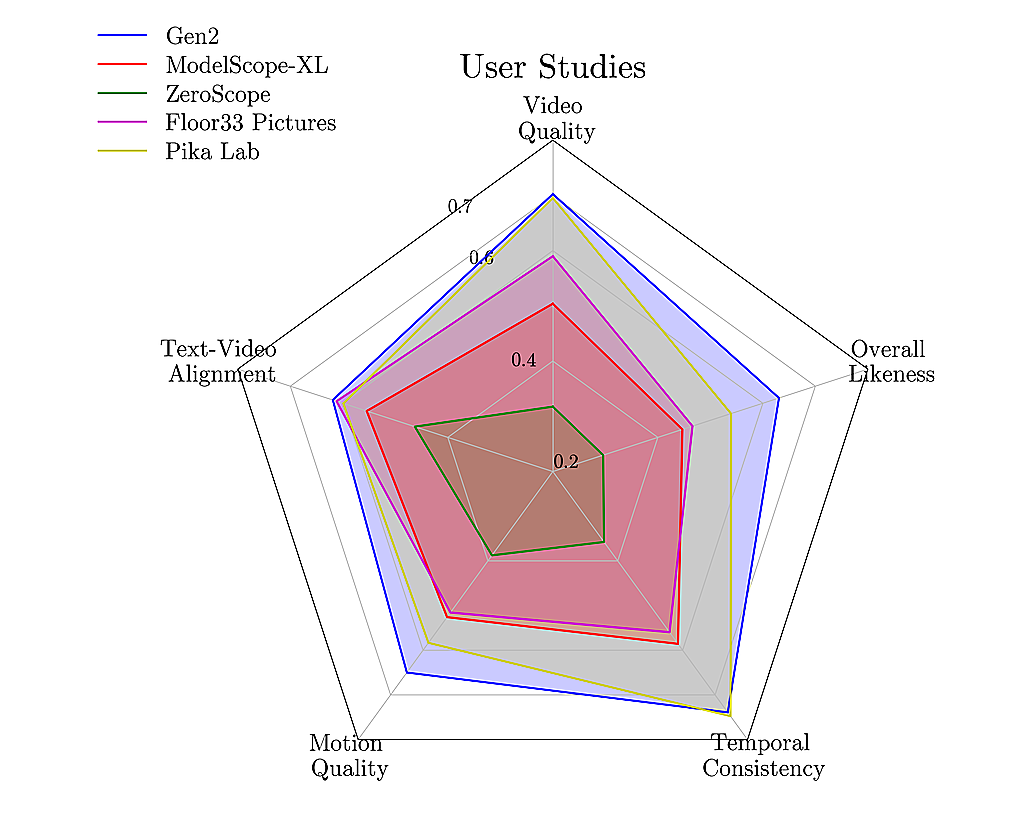
\includegraphics[width=3.300cm,height=2.640cm]{figures/img/results_tiles/evalcrafter_userradar.png}}};
\draw[black!35,line width=0.35pt] (10.140,-5.260) rectangle (13.440,-7.900);
\node[anchor=north west,text=ACMDarkBlue,font=\scriptsize,inner sep=0] at (10.160,-7.920) {\href{https://arxiv.org/abs/2310.11440}{EvalCrafter}};
\node[anchor=north west,text=black!55,font=\tiny,inner sep=0] at (10.160,-8.150) {\href{https://arxiv.org/abs/2310.11440}{arXiv:2310.11440}};
\fill[rgC!82!black] (0,-8.660) rectangle (13.62,-9.160);
\node[anchor=west,text=white,font=\footnotesize\bfseries,inner sep=0] at (0.12,-8.910) {Distributions \& composition};
\node[anchor=north west,inner sep=0] at (0.060,-9.230) {\href{https://arxiv.org/abs/2310.11440}{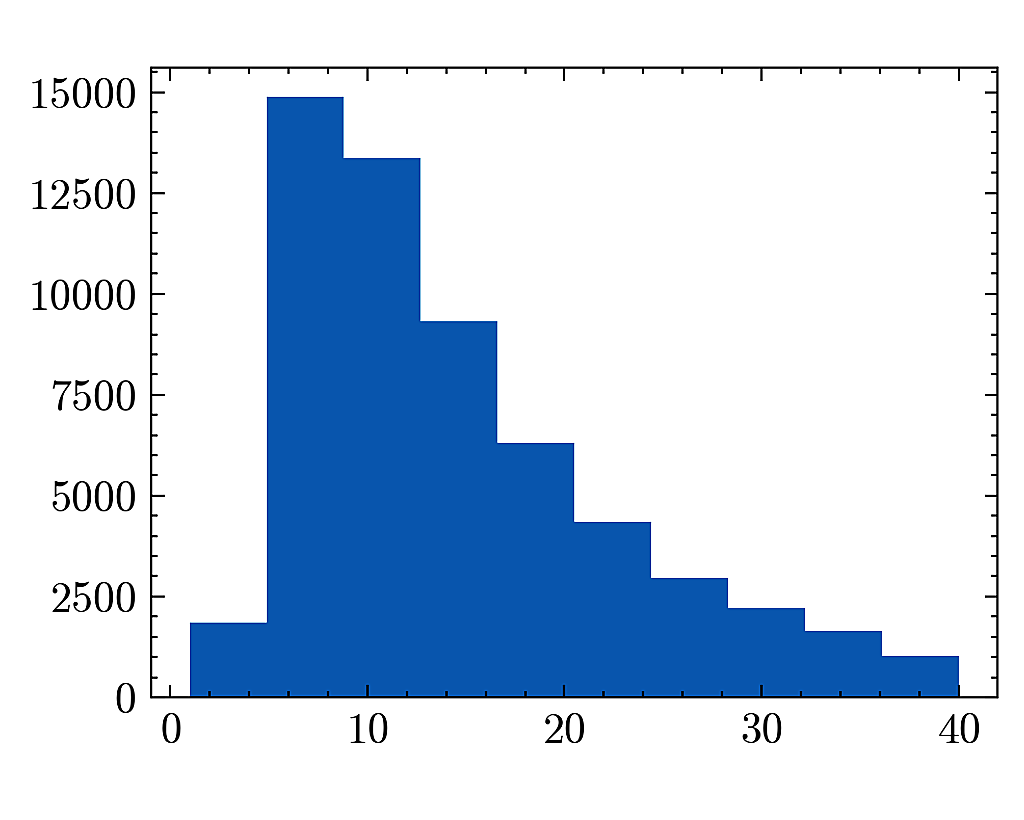
\includegraphics[width=3.300cm,height=2.640cm]{figures/img/results_tiles/evalcrafter_hist.png}}};
\draw[black!35,line width=0.35pt] (0.060,-9.230) rectangle (3.360,-11.870);
\node[anchor=north west,text=ACMDarkBlue,font=\scriptsize,inner sep=0] at (0.080,-11.890) {\href{https://arxiv.org/abs/2310.11440}{EvalCrafter}};
\node[anchor=north west,text=black!55,font=\tiny,inner sep=0] at (0.080,-12.120) {\href{https://arxiv.org/abs/2310.11440}{arXiv:2310.11440}};
\node[anchor=north west,inner sep=0] at (3.420,-9.230) {\href{https://arxiv.org/abs/2310.11440}{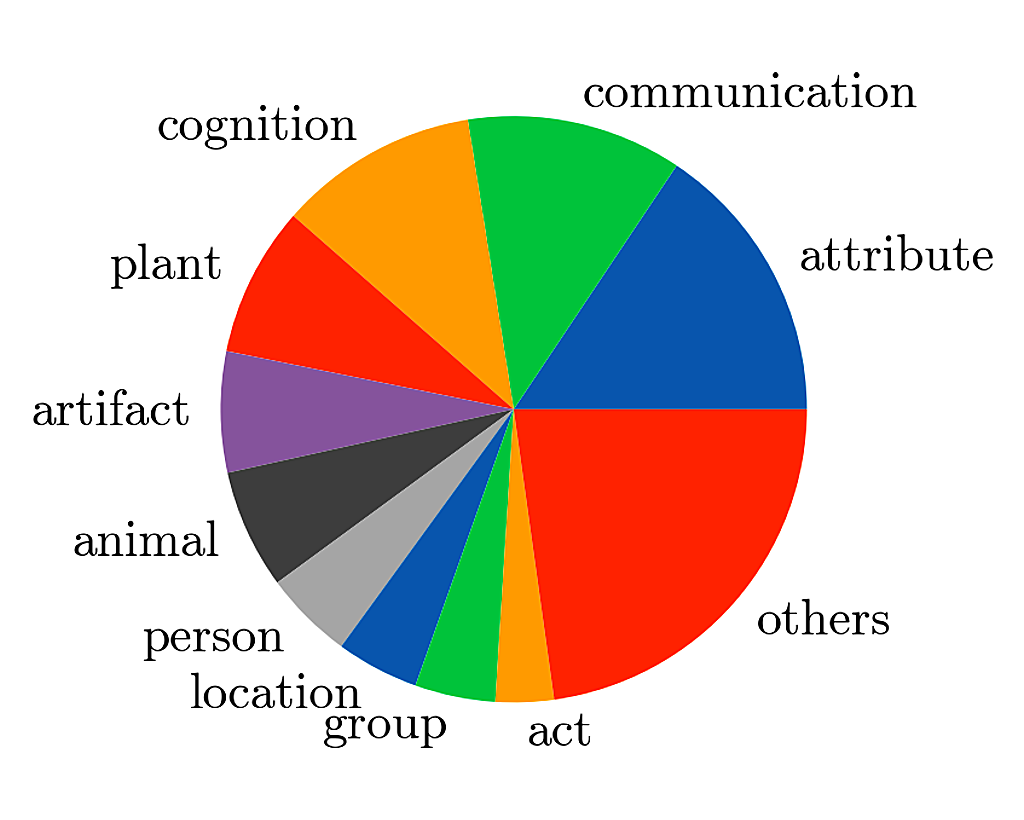
\includegraphics[width=3.300cm,height=2.640cm]{figures/img/results_tiles/evalcrafter_pie.png}}};
\draw[black!35,line width=0.35pt] (3.420,-9.230) rectangle (6.720,-11.870);
\node[anchor=north west,text=ACMDarkBlue,font=\scriptsize,inner sep=0] at (3.440,-11.890) {\href{https://arxiv.org/abs/2310.11440}{EvalCrafter}};
\node[anchor=north west,text=black!55,font=\tiny,inner sep=0] at (3.440,-12.120) {\href{https://arxiv.org/abs/2310.11440}{arXiv:2310.11440}};
\node[anchor=north west,inner sep=0] at (6.780,-9.230) {\href{https://arxiv.org/abs/2311.17982}{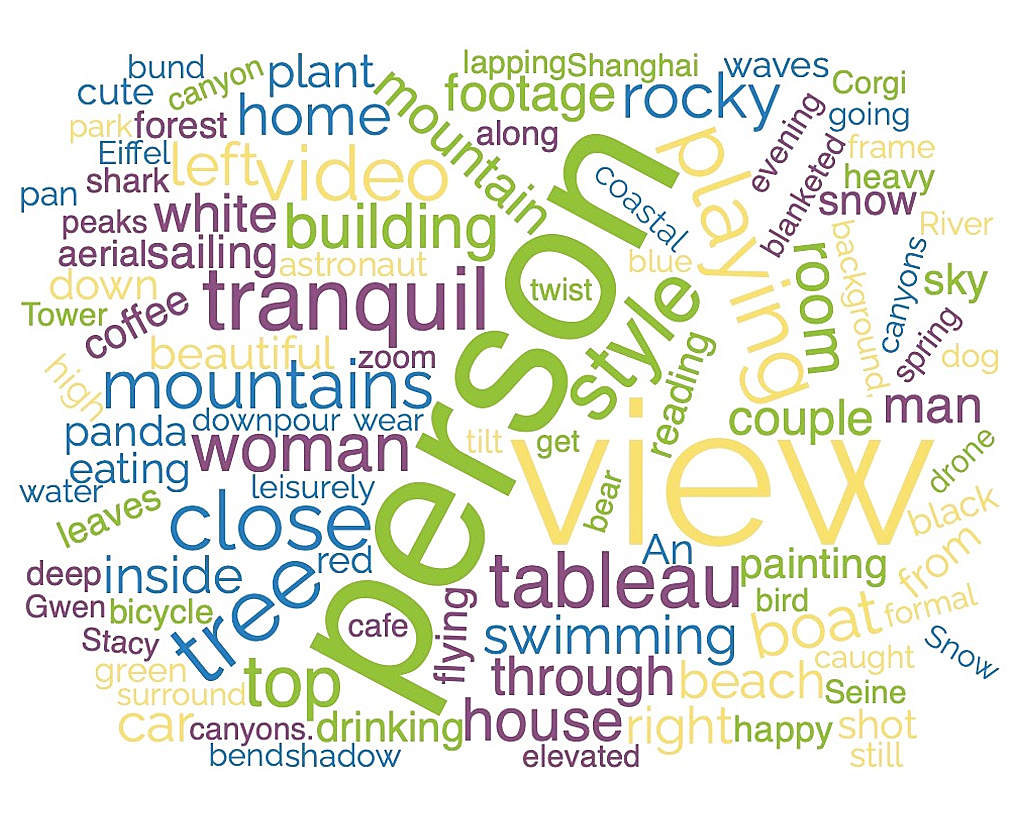
\includegraphics[width=3.300cm,height=2.640cm]{figures/img/results_tiles/vbench_wordcloud.png}}};
\draw[black!35,line width=0.35pt] (6.780,-9.230) rectangle (10.080,-11.870);
\node[anchor=north west,text=ACMDarkBlue,font=\scriptsize,inner sep=0] at (6.800,-11.890) {\href{https://arxiv.org/abs/2311.17982}{VBench}};
\node[anchor=north west,text=black!55,font=\tiny,inner sep=0] at (6.800,-12.120) {\href{https://arxiv.org/abs/2311.17982}{arXiv:2311.17982}};
\node[anchor=north west,inner sep=0] at (10.140,-9.230) {\href{https://arxiv.org/abs/2406.03520}{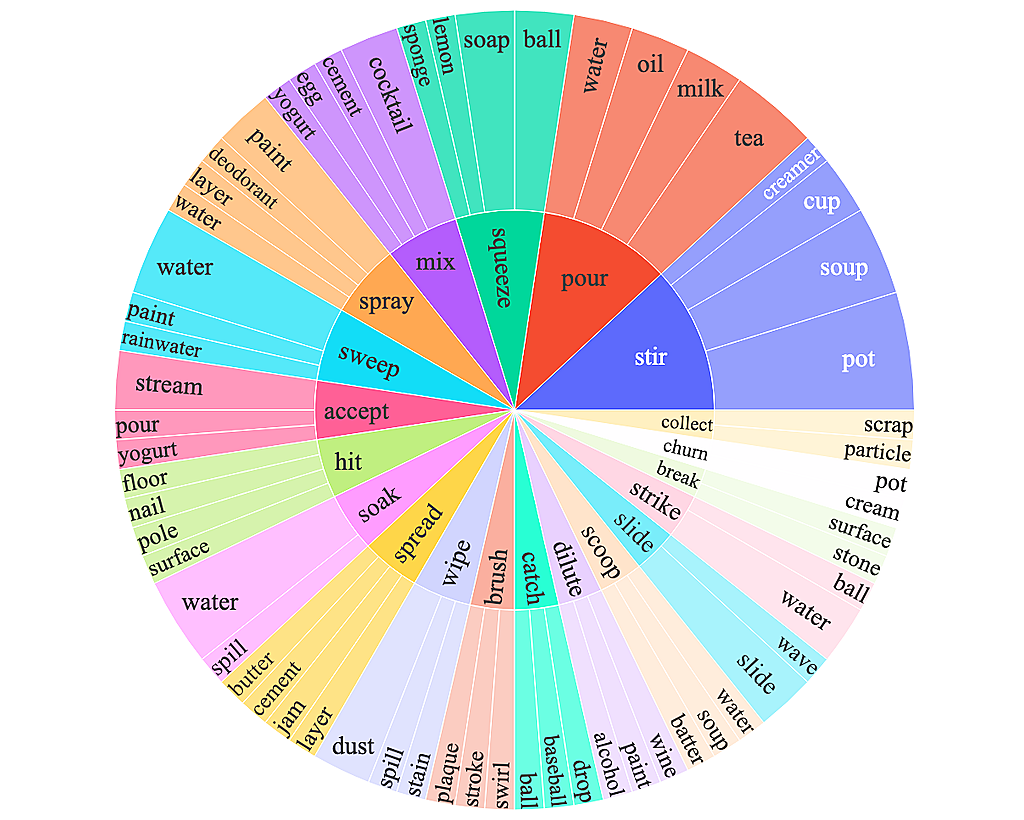
\includegraphics[width=3.300cm,height=2.640cm]{figures/img/results_tiles/videophy_sunburst.png}}};
\draw[black!35,line width=0.35pt] (10.140,-9.230) rectangle (13.440,-11.870);
\node[anchor=north west,text=ACMDarkBlue,font=\scriptsize,inner sep=0] at (10.160,-11.890) {\href{https://arxiv.org/abs/2406.03520}{VideoPhy}};
\node[anchor=north west,text=black!55,font=\tiny,inner sep=0] at (10.160,-12.120) {\href{https://arxiv.org/abs/2406.03520}{arXiv:2406.03520}};
\end{tikzpicture}}
\caption{\textbf{Results reported across the surveyed corpus.} Representative results figures from the catalogue, grouped by type of evidence: \emph{leaderboard and model-comparison charts}, \emph{per-dimension radar and multi-metric} plots, and \emph{distributions and composition}. Each panel is a live hyperlink to the source paper on arXiv and is annotated with its arXiv id (per-panel provenance in Table~\ref{tab:results_provenance}); the figure is vector with plots embedded at full resolution. Only results/leaderboard/metric figures are shown; task and scene figures appear in Figure~\ref{fig:subject_gallery}. As a benchmark survey the reported evidence is dominated by rankings, radars and distributions rather than training curves, and is sparser than the subject figures, so this gallery is smaller; benchmarks that publish no results figure are omitted, not fabricated. A benchmark may appear more than once when it reports several evidence types. Images \textcopyright\ their respective authors, reproduced for scholarly review.}
\Description{A gallery of benchmark results figures in three evidence-type bands. The top band, leaderboard and model-comparison charts, shows four ranking bar charts and win-rate tables. The middle band, per-dimension radar and multi-metric, shows three radar plots over evaluation dimensions. The bottom band, distributions and composition, shows a prompt-length histogram, a meta-type pie chart, and a prompt word cloud. Each panel is labelled with the benchmark name and its arXiv id.}
\label{fig:results_gallery}
\end{figure*}


\subsection{Prediction-to-action bridges}
\label{sec:lane_bridge}

The bridge lane is the frontier, and it is tiny: four benchmarks. RoboWM-Bench~\cite{robowmbench}
tests whether a world model's predictions are \emph{executable}; World-in-World~\cite{worldinworld}
and WorldArena~\cite{worldarena} place world models in a closed loop and score task success rather
than rollout realism; WorldSimBench~\cite{worldsimbench} scores generative models both as renderers
and as controllable simulators. These are the only benchmarks that carry prediction all the way into
executed action, and they are the shaded frontier of Figure~\ref{fig:taxonomy_main}. Even so, none of
the four yet reports a per-capability, head-to-head comparison between a direct VLA policy and a
world-model policy under one protocol. The bridges prove the loop can be closed; they do not yet
close it in a way that isolates the advantage of prediction. That is the gap Section~\ref{sec:gap}
formalises.

\FloatBarrier
